%versi 2 (8-10-2016)\chapter{Landasan Teori}
\chapter{Dasar Teori}
\label{chap:teori}

\section{Privasi}
\label{sec:privasi}
Privasi adalah suatu keadaan dimana kehidupan pribadi seseorang atau sekelompok orang terbebas dari pengawasan atau gangguan orang lain. Privasi juga dapat berarti kemampuan satu atau sekelompok individu untuk menutupi atau melindungi kehidupan dan urusan personalnya dari publik dengan mengontrol sumber-sumber informasi mengenai diri mereka. Untuk melakukan publikasi data dari satu perusahaan ke perusahaan lain, digunakan teknik anonimisasi data untuk melindungi dan menyamarkan atribut sensitif untuk setiap data.

\par Personally Identifiable Information  (PII) adalah standar yang digunakan untuk menentukan apakah informasi yang ada dapat melakukan identifikasi entitas individu secara lansung atau tidak langsung. PII menjelaskan bahwa identifikasi entitas secara langsung dapat dilakukan menggunakan atribut sensitif. Sedangkan identifikasi entitas secara tidak langsung dapat dilakukan menggunakan penggabungan beberapa atribut non-sensitif. PII adalah atribut  yang biasanya terjadi pelanggaran data dan pencurian identitas. Jika data perusahaan atau organisasi terungkap, maka data pribadi pelanggan sangat mungkin terungkap. PII yang diketahui dapat dijual dan digunakan untuk melakukan pencurian identitas, menempatkan korban dalam risiko.
\\\\
Berikut adalah contoh informasi yang bersifat sensitif menurut standar PII:

\begin{itemize}
\item Identitas diri \\ 
Nama lengkap, tempat tanggal lahir, alamat rumah, alamat email.
\item Nomor identitas diri \\
NIK, nomor passport, nomor SIM, nomor wajib pajak, nomor rekening, nomor telepon, dan nomor kartu kredit.
\item Karakteristik pribadi  \\
Foto diri, sidik jari, dan tulisan tangan.
\item Data biometrik \\
Pemindaian retina, jenis suara, dan geometri wajah.
\item Aset informasi lainnya \\
IP Address dan Media Access Control (MAC). 
\end{itemize}

\noindent Berikut adalah contoh informasi yang bersifat non-sensitif menurut standar PII:
\begin{itemize}
\item Rekaman medis
\item Riwayat pendidikan
\item Riwayat pekerjaan 
\item Informasi finasial
\item Letak geografis
\end{itemize}

\newpage
\section{Data Mining}
Data yang dikumpulkan bertambah banyak, sehingga perlu adanya cara untuk melakukan proses ekstraksi informasi pada sekumpulan data yang sangat banyak. Menurut Gartner, Data Mining adalah proses menemukan korelasi, pola, dan tren baru yang bermakna dengan menyaring sejumlah besar data yang disimpan menggunakan teknologi pengenalan pola serta teknik statistik dan matematika. Data mining merupakan bagian dari Knowledge Discovery in Databases (KDD). KDD adalah proses transformasi sekumpulan data yang disimpan pada basis data menjadi informasi yang berguna.\\

\begin{figure}[H]
	\centering
	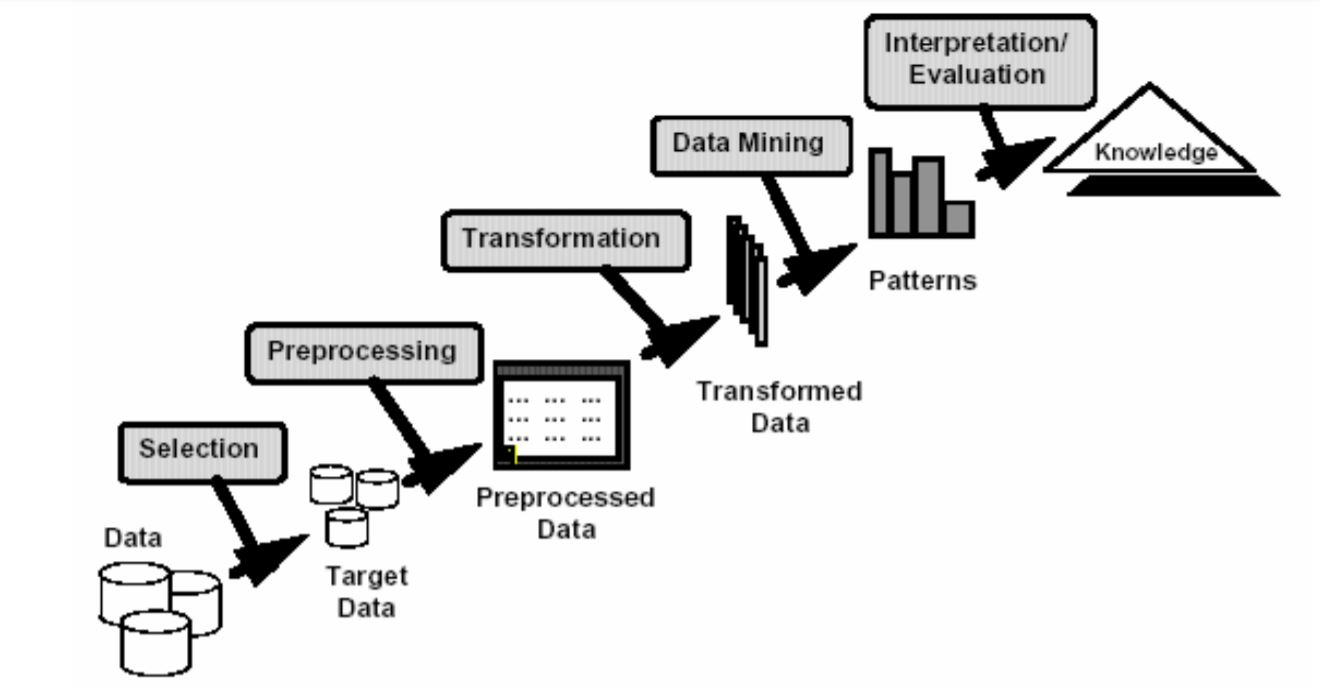
\includegraphics[scale=0.3]{datamining1}
	\caption{Tahapan pada KDD}
	\label{fig:datamining1}
\end{figure}

\noindent Berikut ini adalah penjelasan tahapan pada KDD pada Gambar \ref{fig:datamining1} sebagai berikut:

\begin{enumerate}
\item Selection: proses mengambil data yang relevan terhadap analisis.
\item Preprocessing: proses pembersihan data dari data yang tidak konsisten dan integrasi data saat penggabungan data.
\item Transformation: proses manipulasi data menggunakan konsep agregasi, generalisasi, normalisasi, dan reduksi untuk kebutuhan analisis.
\item Data Mining: proses ekstraksi informasi menggunakan metode pengenalan pola seperti klasifikasi, pengelompokan/clustering.
\item Interpretation/Evaluation: proses interpretasi hasil pengolahan data menjadi sebuah grafik yang dapat dimengerti.
\end{enumerate}


\noindent Berikut adalah beberapa jenis tipe data terkait teknik data mining:

\begin{itemize}

\item Binary: tipe data alphabet/numerik yang hanya memiliki 2 kemungkinan nilai.\\
Contoh: diadakan survei evaluasi beberapa produk pakaian untuk mengetahui produk yang diminati dan tidak diminati. Penilaian produk dapat diwakilkan nilai True atau False. True atau False termasuk jenis binary.

\item Nominal: tipe data alphabet/numerik yang memiliki lebih dari 2 kemungkinan nilai.\\
Contoh: seseorang memilih beberapa bahan dari warna yang berbeda. Warna yang mungkin adalah kuning, hijau, hitam, merah. Warna termasuk jenis nominal.

\end{itemize}

\noindent Tujuan dari penggunaan teknik data mining adalah sebagai berikut:

\begin{itemize}

\item Prediksi: proses menggunakan nilai dari beberapa atribut yang sudah ada untuk memprediksi nilai atribut di masa yang akan datang. Contoh: klasifikasi.

\item Deskripsi: proses menemukan pola yang dapat merepresentasikan kelompok dari sebuah data. Contoh: pengelompokan/clustering.

\end{itemize}

\subsection{Klasifikasi} 
Klasifikasi adalah proses menemukan model (atau fungsi) yang cocok untuk mendeskripsikan dan membedakan sebuah kelas data dengan kelas data lain. Dalam pembelajaran mesin, klasifikasi sering dianggap sebagai contoh dari metode pembelajaran yang diawasi, yaitu menyimpulkan fungsi dari data pelatihan berlabel. \\

\noindent Berikut adalah tahapan klasifikasi secara umum:
\begin{enumerate}

\item
Pelatihan: proses konstruksi model klasifikasi menggunakan algoritma tertentu. Algoritma digunakan untuk membuat model belajar menggunakan set pelatihan data yang tersedia. Model dilatih untuk menghasilkan prediksi yang akurat.

\item
Klasifikasi: model yang digunakan untuk memprediksi label kelas dan menguji model yang dibangun pada data uji dan karenanya memperkirakan akurasi aturan klasifikasi.
\end{enumerate}
\vspace{0.3cm}
\noindent Berikut adalah kategori pemodelan klasifikasi:
\begin{itemize}

\item 
Discriminative: pemodelan paling mendasar untuk menentukan satu kelas untuk setiap baris data. Pemodelan ini bergantung pada data yang diamati dan sangat bergantung pada kualitas data daripada distribusi data.

\begin{figure}[H]
	\centering
	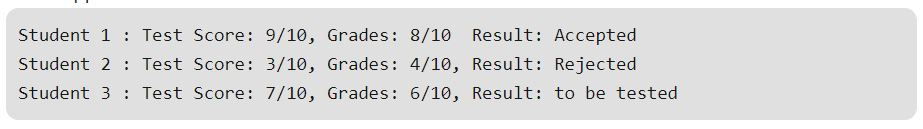
\includegraphics[scale=0.75]{klasifikasi1}
	\caption{Contoh soal}
	\label{fig:klasifikasi1}
\end{figure}

Contoh: Logistic Regression\\
Penerimaan siswa pada sebuah Universitas, untuk mempertimbangkan test score dan grades terhadap keputusan seorang siswa diterima/tidak diterima.

\item 
Generative: pemodelan ini memodelkan distribusi kelas individu dan mencoba mempelajari model yang menghasilkan data dengan memperkirakan asumsi dan distribusi model. Digunakan untuk memprediksi nilai data yang belum diketahui. \\\\
Contoh: Naive Bayes \\
Mendeteksi email spam dengan melihat data sebelumnya. Misalkan dari 100 email yang ada dibagi menjadi kategori Kelas A: 25\% (Email spam) dan Kelas B: 75\% (Email Non-Spam). Ingin diperiksa apakah email berisi  spam atau bukan. Pada Kelas A, 20 dari 25 email adalah spam dan sisanya bukan spam. Pada Kelas B, 70 dari 75 email bukan spam dan sisanya adalah spam. Probabilitas email yang berisi spam termasuk pemodelan naive bayes. \\
\end{itemize}

\noindent Berikut adalah contoh pemodelan yang umum digunakan:
\begin{itemize}
\item Decision Trees
\item Naive Bayes
\item Neural Networks
\item K-Nearest Neighbour
\item Linear Regression
\end{itemize}

\newpage
\subsection{Naive bayes}
\par Naive bayes menerapkan klasifikasi dengan menggunakan metode probabilitas dan statistik. Pemodelan ini mencari nilai probabilitas tertinggi pada masing-masing kelas menggunakan teorema Bayes. Kelas dengan probabilitas tertinggi akan dipilih sebagai hasil akhir. Naive bayes mudah untuk dibangun dan memiliki komputasi yang lebih cepat daripada model klasifikasi lainnya.\\

\noindent Teorema Bayes menemukan probabilitas suatu peristiwa terjadi mengingat probabilitas peristiwa lain yang telah terjadi. Teorema Bayes dinyatakan secara matematis melalui persamaan berikut:

\begin{equation}
P(H|D) = \frac{P(D|H) \cdot P(H)}{P(D)}
\end{equation}

\noindent
Dari perhitungan probabilitas teorema Bayes, akan dicari kelas dengan probabilitas maksimum. Probabilitas maksimum dapat dinyatakan secara matematis melalui persamaan berikut:

\begin{align}
MAP(H) = max(P(H|D))
\end{align}

\noindent Keterangan:
\begin{itemize}
\item P(H|D) adalah probabilitas posterior apabila diberika hipotesis H dan diketahui data D. 
\item P(D|H) adalah probabilitas posterior data D jika hipotesis h adalah benar.
\item P(H) adalah probabilitas hipotesis h adalah benar 
\item P(D) adalah probabilitas data.
\end{itemize}

\vspace{0.3cm}

\noindent Dataset diberikan untuk menggambarkan kondisi cuaca saat bermain golf. Masing-masing data dikategorikan berdasarkan nilai atribut PlayGolf, yaitu cocok ("Yes") atau tidak cocok ("No"). 

\begin{figure}[H]
	\centering
	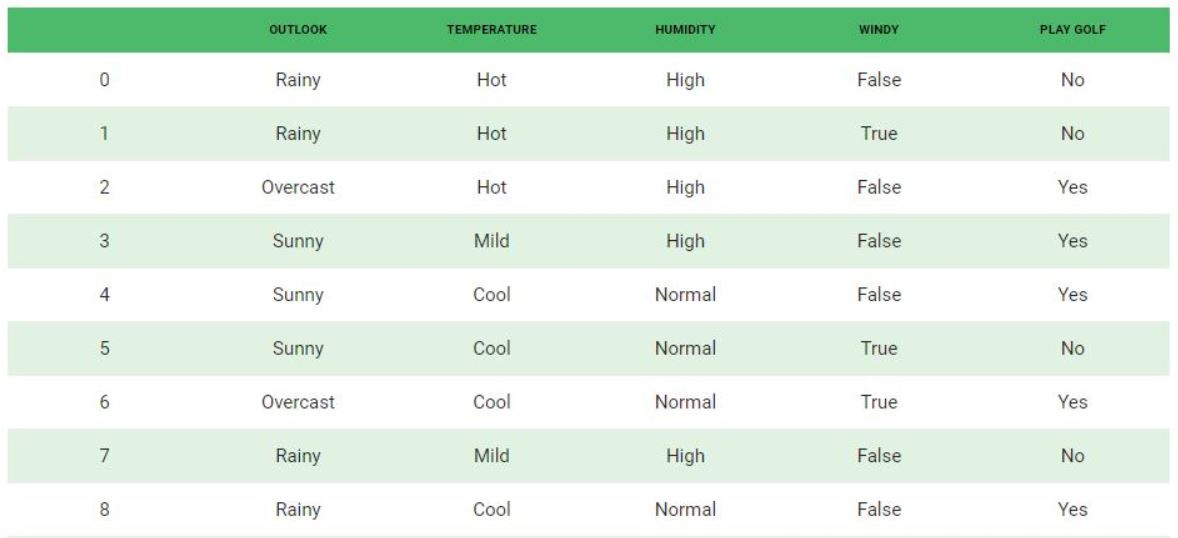
\includegraphics[scale=0.75]{naive_bayes1}
	\caption{Dataset untuk kondisi cuaca saat bermain golf}
	\label{fig:naive_bayes1}
\end{figure}

\noindent Berikut adalah pengelompokan nilai berdasarkan dataset yang telah diberikan:

\begin{itemize}

\item 
Vektor Fitur\\
Vektor Fitur adalah vektor yang mewakili nilai fitur untuk setiap baris dataset. Vektor Fitur dalam dataset ini tersusun dari nilai atribut Outlook, Temperature, Humidity, dan Windy.

\item
Vektor Respon\\
Vektor Respon adalah nilai prediksi kelas untuk setiap vektor fitur. Vektor Respon dalam dataset ini diwakili oleh nilai atribut PlayGolf.

\end{itemize}


\noindent Secara singkat, langkah kerja algoritma Naive Bayes dapat dijelaskan sebagai berikut:

\begin{enumerate}
\item Merepresentasikan teorema Bayes terhadap vektor fitur.\\
Berdasarkan dataset, teorema Bayes dapat diubah seperti berikut:

\begin{equation}
P(y|X) = \frac{P(X|y) \cdot P(y)}{P(X)}
\end{equation}

Dimana y adalah variabel kelas dan X adalah vektor fitur (dengan ukuran n), dinyatakan melalui persamaan berikut:

\begin{equation}
X = (x_1, x_2, x_3, \ldots, x_n)
\end{equation}

Contoh: X = (Rainy, Hot, High, False), y = No
\\\\
Diasumsikan teorema Bayes saling independen terhadap fitur-fiturnya. Berikut adalah persamaan teorema Bayes baru, jika memakai lebih dari satu nilai atribut:

\begin{equation}
P(y|x_1,\ldots,x_n) = \frac{P(x_1|y) P(x_2|y) \ldots P(x_n|y) P(y)}{P(x_1) P(x_2) \ldots P(x_n)}
\end{equation}


\item Menghitung probabilitas masing-masing atribut.

\begin{figure}[H]
	\centering
	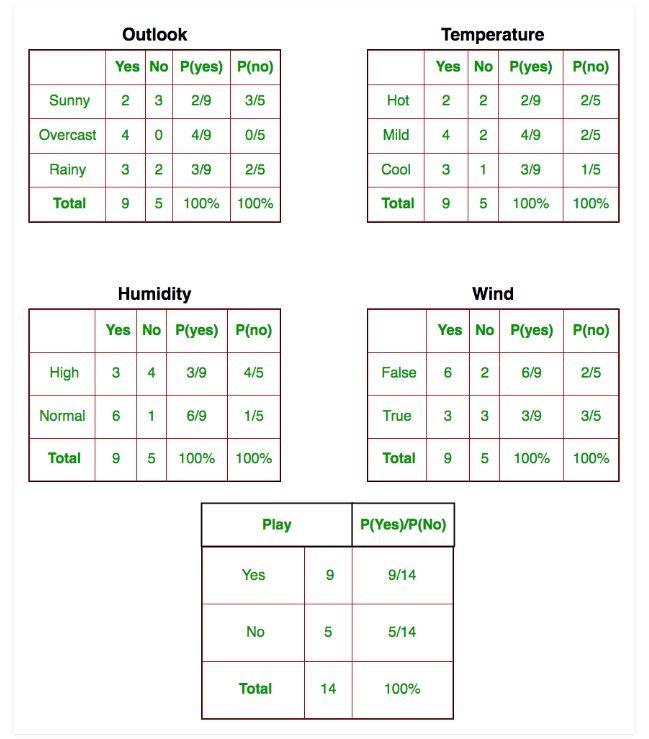
\includegraphics[scale=0.55]{naive_bayes2}
	\caption{Menghitung Probabilitas}
	\label{fig:naive_bayes2}
\end{figure}

Contoh: menghitung $P(No)$ untuk nilai "Sunny" pada atribut "Outlook"
\begin{equation}
P(No) = \frac{frekuensi(Sunny \cap No)}{frekuensi(No)}
\end{equation}

Contoh: menghitung $P(Yes)$ untuk nilai "Sunny" pada atribut "Outlook"
\begin{equation}
P(Yes) = \frac{frekuensi(Sunny \cap Yes)}{frekuensi(Yes)}
\end{equation}

\item Menghitung probabilitas bersyarat jika diketahui nilai dari data baru. \\\\
Contoh: today = (Sunny, Hot, Normal, False)
\begin{figure}[H]
	\centering
	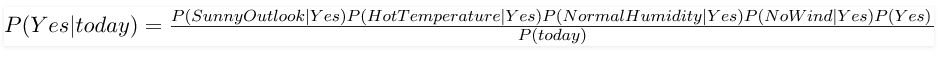
\includegraphics[scale=0.73]{naive_bayes3}
	\label{fig:naive_bayes3}
\end{figure}

\begin{equation}
P(Yes|today) = \frac{3}{5} \cdot \frac{2}{5} \cdot \frac{1}{5} \cdot \frac{2}{5} \cdot \frac{5}{14} = 0.0068
\end{equation}

\begin{figure}[H]
	\centering
	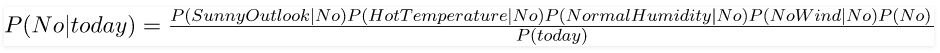
\includegraphics[scale=0.73]{naive_bayes4}
	\label{fig:naive_bayes4}
\end{figure}

\begin{equation}
P(Yes|today) = \frac{2}{9} \cdot \frac{2}{9} \cdot \frac{6}{9} \cdot \frac{6}{9} \cdot \frac{9}{14} = 0.0068
\end{equation}

\item Melakukan normalisasi terhadap probabilitas besyarat.\\

Setelah probabilitas bersyarat dinormalisasi, akan menjadi seperti berikut:

\begin{equation}
P(Yes|today) = \frac{0.0141}{0.0141 + 0.0068} = 0.67
\end{equation}

\begin{equation}
P(Yes|today) = \frac{0.0068}{0.0141 + 0.0068} = 0.33
\end{equation}

Sehingga memiliki probabilitas total seperti berikut:

\begin{equation}
P(Yes|today) + P(No|today) = 1
\end{equation}

\item Mencari probabilitas tertinggi.\\

Berdasarkan pernyataan berikut:
\begin{equation}
P(Yes|today) > P(No|today)
\end{equation}

\noindent Dapat disimpulkan bahwa, jika diberikan data dengan nilai (Sunny, Hot, Normal, False) klasifikasi yang tepat untuk atribut PlayGolf adalah Yes.



\end{enumerate}

\newpage
\subsection{Pengelompokan/Clustering} 
Clustering adalah salah satu teknik analisis data yang paling umum digunakan untuk mendapatkan kemiripan antar data. Clustering dapat didefinisikan sebagai sebuah tugas untuk mengidentifikasi subkelompok dalam data sedemikian rupa sehingga titik data dalam subkelompok yang sama (cluster) sangat mirip sedangkan titik data dalam kelompok berbeda sangat berbeda. Contoh pemodelah clustering adalah K-Means.

\subsection{K-Means} 
K-Means adalah algoritma pembelajaran mesin unsupervised learning untuk menentukan kelompok objek tertentu benar-benar milik. Unsupervised learning artinya tidak ada label yang ditentukan dalam data. Gagasan utama K-Means adalah menetapkan setiap data ke dalam cluster dengan mean terdekat (centroid). Mencari titik terdekat dilakukan dengan cara menghitung distance antara dua data menggunakan Euclidean distance, lalu membandingkat titik yang memiliki jarang paling dekat dengan titik lainnya. \\

\noindent Berikut adalah persamaan untuk menghitung Euclidean distance:
\begin{equation}
EuclidDist(p_i,C_i) = \sqrt[]{(p_1-C_1)^2+(p_2-C_2)^2+\ldots +(p_n-C_n)^2}
\end{equation}
\vspace{0.2cm}

\noindent Diberikan dataset skor A dan B untuk masing-masing individu:

\begin{figure}[H]
	\centering
	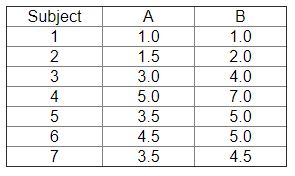
\includegraphics[scale=0.9]{kmeans_1}
	\caption{Contoh Dataset}
	\label{fig:kmeans_1}
\end{figure}

\noindent Secara singkat, langkah kerja algoritma K-Means dapat dijelaskan sebagai berikut:
\begin{enumerate}

\item Kumpulan data ini akan dibuat menjadi dua kelompok dengan menginisialisasi k = 2. Untuk menentukan titik centroid awal, akan dicari nilai A dan B terjauh dengan data lainnya menggunakan Euclidean distance.

\begin{figure}[H]
	\centering
	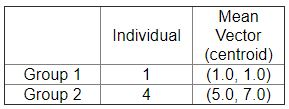
\includegraphics[scale=0.9]{kmeans_2}
	\caption{Hasil Pengelompokan Awal}
	\label{fig:kmeans_2}
\end{figure}

\item Data yang tersisa akan diperiksa secara berurutan dan dialokasikan pada cluster yang paling dekat dengan centroid awal menggunakan Euclidean distance. Vektor rata-rata (centroid) akan dihitung ulang setiap kali anggota baru ditambahkan.

\begin{figure}[H]
	\centering
	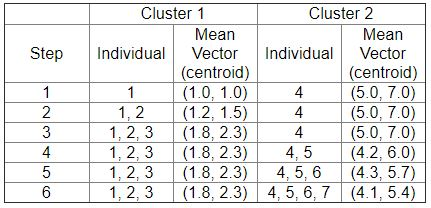
\includegraphics[scale=0.9]{kmeans_3}
	\caption{Mencari Centroid Kelompok}
	\label{fig:kmeans_3}
\end{figure}

\item Menentukan titik centroid baru pada cluster yang baru terbentuk dari tahap sebelumnya.

\begin{figure}[H]
	\centering
	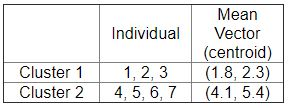
\includegraphics[scale=0.9]{kmeans_4}
	\caption{Hasil Pengelompokan Baru}
	\label{fig:kmeans_4}
\end{figure}

\item Belum bisa dipastikan bahwa setiap individu telah dialokasikan pada cluster yang tepat. Oleh karena itu, perlu membandingkan distance masing-masing data dengan centroid baru pada masing-masing kelompok.

\begin{figure}[H]
	\centering
	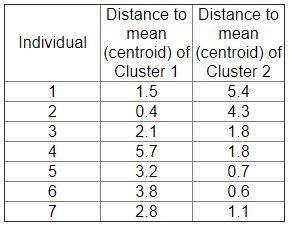
\includegraphics[scale=0.9]{kmeans_5}
	\caption{Euclidean Distance Cluster 1, Cluster 2}
	\label{fig:kmeans_5}
\end{figure}

\item Dapat disimpulkan bahwa, hanya individu 3 yang jaraknya lebih dekat dengan centroid Cluster 2 dari pada centroid Cluster 1. Dengan kata lain, distance masing-masing individu ke centroid kelompoknya sendiri harus lebih kecil daripada rata-rata kelompok lain. Dengan demikian, individu 3 harus dialokasikan ke Cluster 2.

\begin{figure}[H]
	\centering
	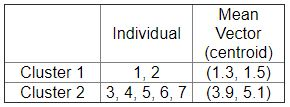
\includegraphics[scale=0.9]{kmeans_6}
	\caption{Hasil Pengelompokan Akhir}
	\label{fig:kmeans_6}
\end{figure}



\end{enumerate}





\newpage
\section{Bidang Terkait Data Mining}
Data mining terhubung dengan beberapa bidang lain seperti statistika, machine learning, pengenalan pola, sistem basisdata, sistem data warehouse, information retrieval, visualisasi data, dan bidang lainnya. Jenis bidang ini memberikan berkontribusi yang signifikan terhadap keberhasilan dalam pengolahan data menggunakan teknik data mining.

\begin{figure}[H]
	\centering
	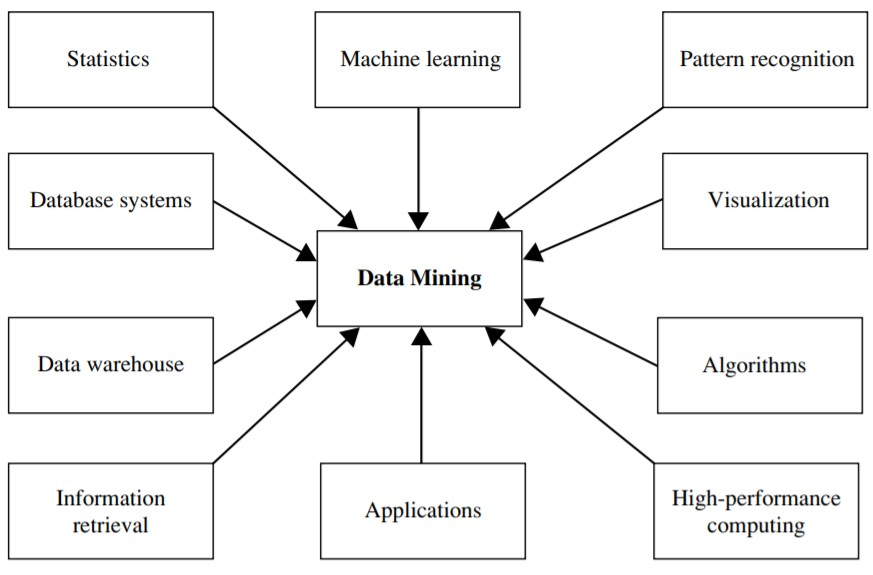
\includegraphics[scale=0.5]{teknologidatamining1}
	\caption{Jenis bidang terkait data mining}
	\label{fig:rnaalgorithm}
\end{figure}

\subsection{Visualisasi Data} 
Visualisasi adalah penggunaan representasi grafik pada komputer. Visualisasi data melibatkan penyajian data dalam bentuk grafik atau gambar agar membuat informasi mudah dimengerti, membantu menjelaskan fakta, dan menentukan arah tindakan.  Dengan adanya representasi data dalam bentuk visual, seseorang dapat memahami sekumpulan data dengan mudah. Hal ini membantu individu  menemukan pola, memahami informasi, dan membentuk opini berdasarkan hasil analisis. 
\\\\
Beberapa teknik visualisasi yang umum digunakan untuk menggambarkan informasi dari sekumpulan data adalah sebagai berikut:

\begin{itemize}
\item Line chart adalah grafik pembanding perubahan nilai atribut pada periode waktu tertentu.
\item Bar chart adalah grafik pembanding nilai atribut untuk jenis kategori yang berbeda.
\item Scatter plot adalah grafik dengan plot dua dimensi yang menunjukkan variasi dua item.
\item Pie chart adalah grafik untuk membandingkan persentase nilai atribut secara keseluruhan.
\end{itemize}

\subsection{Statistika}
Statistika adalah pengetahuan yang berkaitan dengan pengumpulan angka-angka, pengolahan, dan analisis, penarikan kesimpulan, dan membuat keputusan berdasarkan data dan fakta yang sudah dianalisis. Analisis yang dilakukan dalam statistika meliputi ukuran pemusatan dan penyebaran data. Ukuran pemusatan data meliputi nilai rata-rata (mean), modus, dan median. Sedangkan ukuran penyebaran data meliputi variansi dan standar deviasi

\subsubsection{Mean}
Mean adalah nilai rata-rata dari sekumpulan data. Nilai dari mean dapat ditentukan dengan cara membagi jumlah data yang ada dengan total data. Mean terdiri dari dua jenis yaitu: populasi dan sampel. Mean populasi memiliki simbol $\mu$, sedangkan mean untuk sampel memiliki simbol $\overline{x}$.   
\\\\
Berikut adalah persamaan untuk menghitung mean populasi ($\mu$):

\begin{equation}
\mu = \frac{x_1+x_2+x_3+\ldots+x_n}{n}
\end{equation}

\noindent Berikut adalah persamaan untuk menghitung mean sampel ($\overline{x}$):

\begin{equation}
\overline{x} = \frac{x_1+x_2+x_3+\ldots+x_n}{n}
\end{equation}


\subsubsection{Median}
Median menentukan letak dari titik tengah data setelah data disusun menurut urutan nilainya. Median disimbolkan dengan $\widetilde x$. Median dibedakan  berdasarkan jumlah datanya, yaitu jumlah data yang bernilai ganjil dan jumlah data yang bernilai genap. 
\\\\
\noindent Berikut adalah persamaan median untuk jumlah data ganjil dan genap:

\begin{align}
\widetilde x = 
\left\{ \begin{array}{cc} 
X_{\frac{n+1}{2}} & \hspace{5mm} ,n=ganjil \vspace{2mm}\\
\frac{X_{\frac{n}{2}}+X_{\frac{n}{2}+1}}{2}  & \hspace{5mm} ,n=genap \\
 \end{array} 
 \right.
\end{align}

\subsubsection{Modus}
Modus adalah nilai yang sering muncul dalam kelompok data tersebut. Modus berarti nilai data yang memiliki frekuensi terbanyak dalam sekelompok data. 


\subsection{Machine Learning} 
Machine learning mempelajari metode pembelajaran pada sebuah komputer, agar dapat belajar secara mandiri atau meningkatkan kinerjanya berdasarkan data pelatihan yang pernah diberi. Penelitian pada machine learning adalah membuat program komputer bekerja secara otomatis untuk belajar mengenali pola yang kompleks dan membuat keputusan cerdas berdasarkan data. \\

\noindent Berikut adalah contoh pembelajaran pada Machine Learning:

\begin{itemize}

\item
Supervised Learning adalah pembelajaran dengan menggunakan data yang diberi label dengan baik yang berarti beberapa data sudah ditandai dengan jawaban yang benar. Supervised Learning menganalisis data pelatihan dan menghasilkan hasil pelatihan yang benar dari data yang diberi label. Contoh penerapannya adalah clustering.

\item
Unsupervised Learning adalah pembelajaran menggunakan informasi yang tidak diklasifikasikan atau diberi label dan memungkinkan algoritma  bertindak pada informasi tersebut tanpa bimbingan. Unsupervised Learning bertujuan untuk mengelompokkan informasi yang tidak disortir menurut persamaan, pola dan perbedaan tanpa pelatihan data sebelumnya. Contoh penerapannya adalah klasifikasi.

\end{itemize}

\newpage
\section{Privacy Preserving Data Mining (PPDM)} 
Privacy Preserving Data Mining (PPDM) adalah teknik yang telah dikembangkan untuk mencegah pengungkapan informasi sensitif seseorang saat dilakukan data mining dari sekumpulan data yang berukuran besar. PPDM dapat melakukan perubahan dan  menghilangkan sebagian data untuk menjaga privasi. Semakin banyak terjadinya perubahan pada data, maka perlindungan privasi akan meningkat dan kualitas informasi akan menurun.  Utilitas adalah kondisi untuk meningkatkan kualitas informasi yang diperoleh dengan mempertimbangkan jumlah data yang dimodifikasi. Metode PPDM menjamin perlindungan data pada tingkat privasi tertentu bersamaan dengan memaksimalkan utilitas data, sehingga memungkinkan pengolahan data mining menghasilkan informasi yang efektif. Klasifikasi PPDM dibuat berdasarkan siklus pengolahan data mulai dari pengumpulan data, proses data mining, penerbitan data, dan distribusi data.

\subsection{Pengumpulan Data} 
Untuk memastikan privasi tetap terjada pada saat pengumpulan data, perangkat sensor sebagai reseptor input dapat mengacak nilai data yang ditangkap sebelum data dikirimkan kepada kolektor (perangkat lain). Entitas yang mengumpulkan data diasumsikan menjadi entitas yang tidak dapat dipercaya. Oleh karena itu, nilai-nilai data sesungguhnya tidak pernah disimpan dalam basis data, dan nilai-nilai tersebut hanya dapat digunakan setelah melalui tahap transformasi (saat proses KDD). Metode yang dapat digunakan untuk melindungi atribut sensitif saat pengumpulan data adalah randomisation.

\subsection{Proses Data Mining} 
Penambangan data sangat memungkinkan terjadinya identifikasi terhadap atribut sensitif. Berikut adalah beberapa metode yang dapat digunakan untuk melindungi atribut sensitif seseorang saat proses data mining yaitu: association rule hiding adalah aturan untuk mengekstraksi seluruh atribut non-sensitif, downgrading classifier effectiveness adalah teknik untuk menurunkan keakuratan dari classifier yang sering digunakan, query auditing and inference control adalah aturan yang membatasi lingkup penggunaan kueri agregasi berdasarkan dataset, bukan terhadap catatan individu atau kelompok tertentu.

\subsection{Publikasi Data} 
Ada kondisi di mana sebuah perusahaan ingin melakukan publikasi koleksi data baik secara publik atau kepada pihak ketiga untuk analisis data tanpa mengungkapkan kepemilikan data sensitif. Dalam situasi ini, PPDM dapat dicapai dengan melakukan anonimisasi pada atribut data yang bersifat sensitif sebelum data tersebut dipublikasikan. PPDM pada publikasi data dikenal sebagai Privacy Preserving Data Publishing (PPDP). Berikut adalah beberapa metode yang dapat digunakan untuk melindungi atribut sensitif saat publikasi data yaitu: k-anonymity, l-diversity, t-closeness, e-differential privacy.

\subsection{Distribusi Data} 
Ada kondisi di mana seseorang berusaha untuk melakukan teknik data mining melalui data yang bersifat publik, berdasarkan ketehubungan nilai atribut non-sensitif. Beberapa pendekatan dapat digunakan untuk melindungi atribut sensitif saat distribusi data. Pendekatan pertama adalah menggunakan protokol yang aman untuk mencegah pengungkapan atau perhitungan informasi antar entitas seperti: oblivious transfer protocol dan homomorphic encryption.  Pendekatan kedua adalah mempertimbangkan sekumpulan operasi primitif yang sering digunakan pada algoritma data mining seperti: secure sum, secure set union, secure size of intersection, scalar product and the set intersection.

\section{Jenis Serangan Publikasi Data} 
Menurut Dalenius (1977), perlindungan privasi tidak akan memberikan kesempatan bagi orang lain untuk mendapatkan informasi sensitif spesifik dari seseorang atau individu meskipun orang lain mengetahui informasi umum yang berhubungan dengan informasi sensitif individu tersebut. Secara umum, orang lain dapat menemukan sebuah cara untuk memetakan sebuah data ke dalam tabel yang telah dianonimisasi ketika data tersebut telah dipublikasikan. Serangan ini dikenal dengan nama linkage attack. Model serangan ini dapat dikategorikan menjadi dua macam, berdasarkan jenis serangannya.

\subsection{Record Linkage}
Record linkage mengacu pada pemetaan beberapa data korban yang ditargetkan ke dalam sebuah tabel yang dirilis secara publik berdasarkan prinsip anonimisasi. Jika pada proses identifikasi salah satu nilai tupel cocok dengan nilai tupel lainnya pada tabel yang sudah dipublikasi, maka memungkinkan atribut sensitif miliki seseorang dapat diketahui oleh orang lain. Menggunakan pemodelan k-anonimity, terbukti dapat menghindari jenis serangan record linkage.

\subsection{Attribute Linkage} 
Dalam serangan ini, penyerang mendapatkan beberapa informasi terkait atribut sensitifnya, meskipun penyerang tidak dapat menghubungkan satu tupel dengan tupel lain dari data yang telah dipublikasi. Pemodelan  l-diversity dapat mencegah serangan attribute linkage. Kondisi yang diperlukan adalah kesetaraan setidaknya sebuah tupel memiliki l nilai atribut yang berbeda dengan tupel lainnya pada data yang telah dipublikasi. Konsep dasarnya adalah menghindari hubungan atribut jika akan ada nilai sensitif yang bernilai unik pada tupel-tuper tertentu dalam sebuah tabel.

\section{Anonimisasi}
\label{sec:anonimisasi}
Anonimisasi adalah proses menghilangkan pengidentifikasi pribadi, baik langsung maupun tidak langsung, yang dapat menyebabkan seseorang diidentifikasi. Seseorang dapat diidentifikasi secara langsung dari nama, alamat, kode pos, nomor telepon, foto atau gambar, atau beberapa karakteristik pribadi unik lainnya. Seseorang dapat diidentifikasi secara tidak langsung ketika informasi tertentu dihubungkan bersama dengan sumber informasi lain.
\\\\
Berikut adalah beberapa istilah yang umum digunakan pada proses anonimisasi data: 

\begin{itemize}
\item Identifier (ID) adalah atribut yang unik dan secara langsung dapat mengidentifikasi seseorang seperti nama, nomor ID, dan nomor ponsel.
\item Quasi-Identifier (QID) adalah kombinasi atribut yang mungkin terjadi untuk mengidentifikasi individu berdasarkan penggabungan informasi lain dari luar. Seluruh atribut data terkecuali atribut identifier dapat dianggap sebagai atribut quasi-identifier.
\item Equivalence class (EQ) adalah himpunan tupel 
dengan jenis nilai atribut yang identik satu sama lain.
\item Sensitive Attribute (SA) adalah atribut yang menyangkut informasi privasi sensitif seseorang.
\item Non-sensitive Attribute (NSA) adalah atribut yang tidak menyangkut informasi privasi sensitif seseorang.
\end{itemize}

\newpage
\subsection{Anonimisasi berdasarkan generalisasi dan supresi}
Idenya adalah meningkatkan jumlah equivalence class pada tabel dengan mengurangi nilai akurasi data dari atribut quasi-identifier. Quasi-identifier dikategorikan menjadi atribut numerik dan kategorial. Atribut numerik digeneralisasi secara interval, misalnya usia 16 dapat digeneralisasi pada interval [10-20]. Atribut kategorial mengubah nilai asli ke nilai yang lebih umum, misalnya negara "China" digeneralisasi menjadi "Asia". Supresi dipandang sebagai bentuk generalisasi yang ekstrem, karena menghilangkan beberapa nilai atribut.

\subsection{Anonimisasi berdasarkan generalisasi}
Saat ini, banyak jenis algoritma yang dipakai untul implementasi  anonimisasi. Berdasarkan perspektif, metode generalisasi dapat dibagi menjadi global generalization dan local generalization. 

\subsection{Anonimisasi berdasarkan clustering}
Anonimisasi dapat diimplementasikan dengan konsep clustering. Ide dasarnya adalah menghasilkan setidaknya k buah data. Data dalam kelompok yang sama harus semirip mungkin agar kehilangan informasi dapat diminimalkan setelah dilakukan generalisasi. Konsep ini menjadi ide dasar untuk perancangan model K-anonimity.

\section{Hierarchy Based Generalization} 
Hierarchy-based generalization adalah tahapan anonimisasi setelah data yang memiliki quasi-identifier yang sama dikelompokan ke dalam kelas yang sama. Hierarchy-based generalization menggunakan konsep generalisasi dan supresi dalam melakukan anonimisasi. Hierarchy-based generalization termasuk metode full-domain generalization. Full-domain generalization diusulkan oleh Samarati dan Sweeney untuk memetakan seluruh domain untuk masing-masing atribut quasi-identifier pada tabel ke domain yang lebih umum.

\par Full-domain generalization menetapkan bahwa metode generalisasi dapat dilakukan jika quasi-identifier telah ditentukan sebelumnya. Sebagai contoh QI = $\{A_1, \ldots , A_n\}$, dimana A adalah atribut dari tabel dataset. Full-domain generalization digunakan oleh K-Anonymity  untuk menentukan generalisasi dan supresi dari sebuah nilai. Terdapat dua jenis hierarki pada Full-domain generalization yaitu Domain Generalization Hierarchy (DGH) dan Value Generalization Hierarchy (VGH). Jenis hierarki yang paling umum digunakan adalah DGH. Tidak terdapat aturan khusus untuk memodelkan hierarki DGH. Semua nilai atribut dalam tabel harus bisa digeneralisasi menggunakan DGH. DGH adalah konsep sederhana dari penggantian nilai berdasarkan nilai yang kurang spesifik menjadi nilai lebih umum terhadap nilai aslinya. 

Pada Gambar \ref{fig:DGH1}, nilai ZIP \{02138, 02139\} dapat digeneralisasi menjadi \{0213*\} dengan menghilangkan digit paling kanan. Secara semantik nilai yang telah digeneralisasi akan memiliki lingkup nilai yang lebih besar. Pada basis data relasional, domain digunakan untuk merepresentasikan nilai dari masing-masing atribut. Gagasan tentang domain akan diperluas agar lebih mudah dalam memahami cara kerja generalisasi. Dalam basis data, nilai telah dicatat secara spesifik sehingga dapat diasumsikan nilai atribut masih berada pada domain dasar. Sebagai contoh, nilai ZIP adalah \{02138, 02139\} berada pada domain dasar yaitu $Z_0$. Untuk mencapai perlindungan pada K-Anonymity, maka kode ZIP yang sebelumnya representatif harus diubah menjadi kurang informatif. Sebuah nilai dapat digeneralisasi jika memiliki domain yang lebih umum. Sedangkan domain yang kurang spesifik dapat digunakan untuk mendeskripsikan garis besar nilai ZIP. Sebagai contoh dari domain kurang spesifik adalah $Z_1$, di mana digit terakhir diganti dengan simbol (*). Berikut adalah contoh pemetaan dari Z0 ke Z1 seperti berikut $02139 \rightarrow 0213*$.

\newpage
Jika diberikan atribut A, maka fungsi generalisasi untuk atribut A adalah f: $A \rightarrow B$. Gambar 2.1 menyatakan urutan generalisasi secara fungsional dengan definisi fungsi sebagai berikut $f_h$: h = \{$0,\ldots, n-1\}$, sehingga A = $A_0$ and |$A_n$| = 1. Fungsi $f_h$ menerapkan urutan linier pada $A_h$ di mana elemen minimal harus berada pada domain dasar yaitu $A_0$ dan elemen maksimalnya harus berada paling atas yaitu $A_n$. Persyaratannya adalah $A_n$ memastikan bahwa semua nilai yang terkait dengan suatu atribut bisa digeneralisasikan ke nilai tunggal. $A_h$, $h = 0, \ldots, n$ akan diuraikan jika pada implementasi nilainya bertentangan dengan memiliki nilai yang sama. Hubungan seperti itu menyiratkan adanya hierarki generalisasi nilai VGHA untuk atribut A. 

\[
  A_0 \overset{f_0} {\longrightarrow} A_1 \overset{f_1} {\longrightarrow} \mathcal{\ldots} \overset{f_n-1}{\longrightarrow} A_n
\]

Representasi generalisasi diperluas agar metode supresi dapat diterapkan dengan cara membuat hirarki generalisasi untuk elemen dengan nilai maksimal yang baru berada di atas elemen dengan nilai maksimal yang lama. Elemen maksimal baru adalah nilai supresi atribut. Ketinggian setiap hierarki generalisasi akan bertambah seiring munculnya elemen maksimal yang baru. Setelah elemen mencapai nilai maksimal yang dapat digeneralisasi maka tidak akan ada lagi perubahan yang diperlukan untuk memasukkan nilai supresi (*). Gambar \ref{fig:DGH1} dan Gambar \ref{fig:DGH2} memberikan contoh hierarki generalisasi dari nilai dan domain yang diperluas untuk memasukkan elemen maksimal yang disupresi (*****). Pada contoh ini, domain $Z_0$ mewakili kode ZIP untuk Cambridge, MA, dan $E_0$ mewakili ras. Mulai sekarang, semua referensi untuk generalisasi termasuk elemen maksimal baru dan hierarki mengacu pada hierarki generalisasi domain.

\begin{figure}[H]
	\centering
	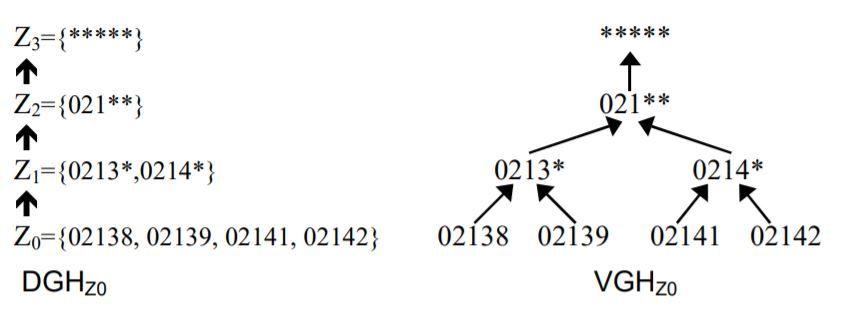
\includegraphics[scale=0.6]{DGH1}
	\caption{DGH dan VGH pada atribut ZIP}
	\label{fig:DGH1}
\end{figure}

\begin{figure}[H]
	\centering
	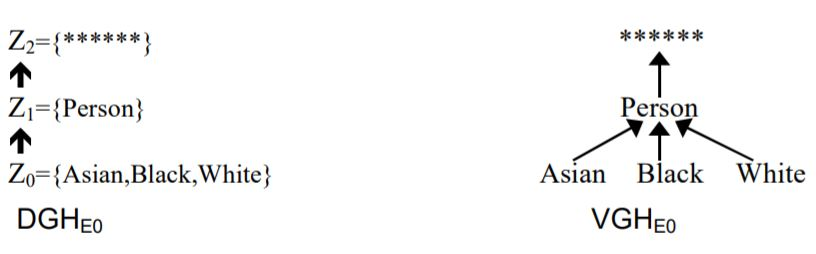
\includegraphics[scale=0.6]{DGH2}
	\caption{DGH dan VGH pada atribut Race}
	\label{fig:DGH2}
\end{figure}




\newpage
\section{K-Anonymity}
K-anonymity merupakan model yang paling efektif untuk melindungi privasi saat melakukan publikasi data. K-anonymity adalah pemodelan untuk mengurangi perbedaan antara satu data dengan data lain, agar sebuah data tidak dapat dibedakan setidaknya dengan k-1 data lainnya. Dengan kata lain, penyerang tidak dapat mengidentifikasi identitas dari satu data karena k-1 data yang lain memiliki sifat yang sama. Dalam pemodelan k-anonymity, nilai k dapat digunakan sebagai tingkat keamanan privasi. Semakin tinggi nilai k, semakin sulit untuk mengindentifikasi sebuah data. Secara teori, probabilitas identifikasi sebuah data adalah 1 / k. Namun, meningkatkan nilai k juga berpengaruh terhadap nilai informasi yang diperoleh dari sekumpulan data.

\par K-Anonymity pertama kali diusulkan pada tahun 1998 oleh Sweeney et al. K- anonymity tergantung pada menganonimkan kumpulan data asli untuk memenuhi persyaratan anonimisasi, yang dapat digunakan untuk penerbitan data. Teknik anonimisasi yang umum adalah generalisasi dan disembunyikan. Gagasan dasar K- anonymity adalah menganonimkan data penerbitan untuk memenuhi persyaratan bahwa setidaknya K buah record yang tidak dapat dibedakan satu sama lain. Yaitu, untuk masing-masing tuple terdapat setidaknya K tuple dengan nilai yang sama dari quasi-identifiers. Para peneliti telah membuktikan bahwa kompleksitas K- anonymity adalah NP-hard. NP-hard adalah istilah yang sering digunakan untuk menyatakan kompleksitas sebuah algoritma sangat tinggi (eksponensial).

\par Penelitian menunjukkan bahwa sebagian besar pemodelan k-anonymity menggunakan metode generalisasi dan supresi. Pendekatan tersebut menderita kehilangan informasi yang signifikan karena mereka sangat bergantung terhadap hubungan relasi antar atribut. Oleh karena itu, hasil anonimisasi menghasilkan nilai kehilangan informasi yang cukup tinggi. Selain itu, algoritma anonimisasi yang ada hanya berfokus pada perlindungan informasi pribadi dan mengabaikan utilitas data yang sebenarnya. Akibatnya, nilai utilitas pada data yang telah dianonimisasi memiliki bernilai rendah. Beberapa algoritma telah dicoba untuk mengimplementasikan pemodelan K-Anonymity.

\par Algoritma k-means clustering akan melakukan beberapa iterasi sampai centroid dari semua data tidak lagi berubah atau perubahannya kecil. Algoritma k-means clustering tidak mampu untuk menyelesaikan masalah pada atribut yang bernilai kategorikal. Kelebihan dari algoritma k-means clustering adalah memiliki hasil pengelompokan yang sudah baik. Kekurangan dari algoritma k-means clustering adalah pemilihan centroid awal k-means secara acak, sehingga setelah digeneralisasi hasil pengelompokannya mengakibatkan hilangnya informasi yang besar.

\par Algoritma k-member dapat melakukan generalisasi atribut kategorikal dengan memperoleh kualitas informasi yang lebih baik daripada algoritma k-means clustering. Namun algoritma k-member masih memiliki masalah ketika melakukan pengelompokan data. Kekurangan dari algoritma K-member adalah hanya mempertimbangkan pengelompokan terakhir tanpa memperhatikan pengelompokan yang dihasilkan pada proses sebelumnya sehingga menyebabkan distribusi kelompok pada beberapa bagian menjadi kurang tepat. 

\par Untuk menghindari kekurangan pada algoritma k-means dan algoritma k-member maka kedua konsep ini perlu digabung menjadi sebuah algoritma baru dengan nama algoritma Greedy K-member Clustering. Algoritma Greedy K-member Clustering mendapatkan hasil pengelompokan yang lebih tepat dan memiliki nilai informasi yang lebih baik meskipun dilakukan generalisasi. Menggunakan algoritma Greedy K-Member Clustering, pengelompokan data dapat dilakukan satu kali sehingga dapat menurunkan kompleksitas algoritma dan hasil  pemilihan centroid dapat dioptimalkan sehingga hasil pengelompokan dapat ditingkatkan secara signifikan. Hasil akhir dari algoritma Greedy K-member Clustering adalah data-data yang sejenis sudah dikelompokan pada kelompok data yang sama. Untuk melakukan anonimisasi pada pemodelan k-anonymity, digunakan konsep Hierarchy Based Generalization. Konsep ini menyamarkan data yang  memiliki nilai quasi-identifier yang sama. Beberapa pemodelan yang dapat digunakan adalah Domain Generalization Hierarchy (DGH) dan Value Generalization Hierarychy (VGH). Pemodelan VGH akan diterapkan pada data yang nilainya sama dengan data lain dalam satu kelompok. 


\section{Greedy K-Member Clustering}
\label{sec:greedyclustering}
Penelitian menunjukkan bahwa sebagian besar metode K-Anonymity didasarkan pada generalisasi dan teknik penekanan sehingga menderita dari kehilangan informasi yang signifikan. Masalah pengelompokan dapat meminimalkan kehilangan informasi melalui algoritma K-Member Clustering. Akan tetapi algoritma K-Member Clustering berpotensi memiliki kompleksitas yang eksponensial. Untuk menurunkan kompleksitas tersebut, maka permasalahan algoritma K-Member Clustering dapat didefinisikan sebagai permasalahan algoritma Greedy. Algoritma Greedy K-Member Clustering bertujuan untuk membagi seluruh tuple pada dataset ke masing-masing cluster dengan kompleksitas yang lebih baik dan mendukung informasi yang lebih banyak dibandingkan algoritma clustering yang lain.

\begin{theorem}
Masalah pengambilan keputusan pada k-member clustering adalah NP-complete.
\end{theorem}

\begin{proof}
Melalui pengamatan Aggarwal et al, permasalahan k-member clustering dapat diselesaikan dengan kompleksitas polinomial.
\end{proof}

\begin{theorem}
N adalah total tuple dan k adalah parameter anonimisasi. Setiap kluster yang ditemukan oleh algoritma greedy k-member clustering memiliki jumlah tuple minimal sebanyak k, dan jumlah tuple tidak melebihi $2k - 1$.
\end{theorem}

\begin{proof}
S adalah himpunan tuple. Algoritma ini menemukan cluster selama jumlah tuple yang tersisa sama dengan atau lebih besar dari k, setiap cluster berisi k tuple. Jika total tuple pada S kurang dari k, maka sisa tuple akan dikelompokan pada kelompok kluster yang sudah ada. Oleh karena itu, ukuran maksimum sebuah cluster adalah $2k - 1$.
\end{proof}

\begin{theorem}
N adalah jumlah tuple dan k menjadi parameter anonimitas yang ditentukan. Jika $n > k$, kompleksitas algoritma greedy k-member clustering adalah $O(n^2)$.
\end{theorem}

\begin{proof}
Algoritma greedy k-member clustering menghabiskan sebagian besar waktunya untuk memilih tuple dari S satu per satu hingga mencapai $|S| = k$. Karena ukuran set input berkurang satu pada setiap iterasi, total waktu eksekusi adalah O $(n^2)$.
\end{proof}

\noindent Beberapa hal penting terkait algoritma Greedy K-Means Clustering:

\begin{itemize}
\item Menetapkan tabel S  
\item Menetapkan nilai k
\item Menetapkan jumlah cluster (m) yang ingin dibuat
\begin{align}
m = \left \lfloor \frac{n}{k} \right \rfloor - 1
\end{align}
\end{itemize}


\noindent Berikut adalah langkah kerja algoritma Greedy K-Means Clustering secara lengkap:

\begin{enumerate}
\item Melakukan inisialisasi variabel result dengan himpunan kosong dan variabel r dengan memilih data secara acak dari tabel S

\item Pada kondisi $|S| \geq k$, lakukan perulangan sebagai berikut:

\begin{enumerate}
\item Memilih data baru pada variabel r berdasarkan perbedaaan distance tertinggi dari nilai r sebelumnya. Perbedaan distance dapat dicari menggunakan rumus berikut:
\begin{align*}
\Delta (r_1,r_2) = \sum_{i=1}^{m} \delta_N(r_1[N_i],r_2	[N_i]) +  \sum_{j=1}^{n} \delta_C(r_1[C_j],r_2[C_j])
\end{align*}

\noindent Berikut adalah rumus menghitung distance antar data numerik:
\begin{align*}
\delta_n(v_1,v_2) = \frac{|v_1 - v_2|}{|D|} 
\end{align*}

\vspace{0.4cm}

\noindent Berikut adalah rumus menghitung distance antar data kategorikal:

\begin{align*}
\delta_C(v_1,v_2) = \frac{H(\Lambda(v_i,v_j))}{H(T_D)} 
\end{align*}

\vspace{0.4cm}

\item Membuang himpunan data variabel r pada variabel S

\item Mengisi data dari variabel r pada variabel c.

\item Pada kondisi $|c| \geq k$, lakukan perulangan sebagai berikut:

\begin{enumerate}
\item Memilih data baru terbaik untuk variabel r berdasarkan nilai Information Loss (IL) yang paling rendah. Information Loss (IL) dapat dicari menggunakan rumus berikut:

\begin{align*}
IL(e)&= |e| \cdot D(e) \\
D(e) &= \sum_{i=1}^{m} \frac{(MAX_{N_i} - MIN_{N_i})}{|N_i|} + \sum_{j=1}^{n}\frac{H(\Lambda(\cup_{C_j}))}{H(T_{C_j})}
\end{align*}

\item Membuang himpunan data dari variabel r pada variabel S

\item Menambahkan himpunan data dari variabel r pada variabel c.

\item Menambahkan himpunan data dari variabel c pada variabel result

\end{enumerate}

\end{enumerate}

\item Pada kondisi $|S| \neq  0$, artinya jika masih terdapat data yang belum dimasukkan pada sebuah cluster dari tabel S, lakukan perulangan sebagai berikut:

\begin{enumerate}
\item Memilih data secara acak dari tabel S untuk disimpan pada variabel r

\item Membuang himpunan data dari variabel r pada variabel S

\item Memilih cluster terbaik untuk variabel c berdasarkan nilai Information Loss (IL) yang paling rendah. Information Loss (IL) dapat dicari menggunakan rumus berikut:

\begin{align*}
IL(e)&= |e| \cdot D(e) \\
D(e) &= \sum_{i=1}^{m} \frac{(MAX_{N_i} - MIN_{N_i})}{|N_i|} + \sum_{j=1}^{n}\frac{H(\Lambda(\cup_{C_j}))}{H(T_{C_j})}
\end{align*}

\item Menambahkan himpunan data dari variabel r pada variabel c.

\end{enumerate}

\item Algoritma ini mengembalikan himpunan data berdasarkan jenis cluster yang berbeda-beda melalui variabel result.

\end{enumerate}

\newpage
\noindent Berikut adalah pseudocode secara lengkap dari algoritma greedy k-member clustering:

\begin{algorithm}[H]
  \caption{Find Best Record}\label{alg:1}
  \begin{algorithmic}[1]
  %-------------- Input & Output -----------------
  \State \textbf{Function} \texttt{find\_best\_record(S,c)}
  \State \textbf{Input:} a set of records S and a cluster c.
  \State \textbf{Output:} a record r $\in$ S such that $IL(c \cup \{r\})$ is minimal
  \\
  %-------------- Baris 1-3 -----------------
  \State{$n = |S|$}
  \State{$min = \infty$}
  \State{$best = null$}
  \For{$i = 1 \ldots n$}
  \State{r = i-th record in S}
  \State{diff = $IL(c \cup \{r\}) - IL(c)$}
  \If{diff < min}
  \State{min = diff}
  \State{best = r}
  \EndIf
  \EndFor
  \State{return best}
  \end{algorithmic}
\end{algorithm}
Algoritma \ref{alg:1} menerima input himpunan data  dataset dan sebuah data dengan nilai distance tertinggi dari data terpilih acak. Algoritma ini menghitung selisih distance dari dua jenis data yang berbeda. Variabel "diff" pada algoritma ini adalah perbedaan distance, dicari dengan penjumlahan information loss pada sebuah kluster dengan information loss pada data ke-i, lalu hasil penjumlahan tersebut dikurangi dengan information loss dari kluster. Output algoritma ini adalah sebuah data dengan nilai terbaik, yaitu data ke-i dari dataset S dengan nilai distance paling kecil.
\begin{algorithm}[H]
  \caption{Find Best Cluster}\label{alg:2}
  \begin{algorithmic}[1]
  %-------------- Input & Output -----------------
  \State \textbf{Function} \texttt{find\_best\_cluster(C,r)}
  \State \textbf{Input:} a set of cluster C and a record r.
  \State \textbf{Output:} a cluster c $\in$ C such that $IL(c \cup \{r\})$ is minimal
  \\
  %-------------- Baris 1-3 -----------------
  \State{$n = |C|$}
  \State{$min = \infty$}
  \State{$best = null$}
  \For{$i = 1 \ldots n$}
  \State{c = i-th cluster in C}
  \State{diff = $IL(c \cup \{r\}) - IL(c)$}
  \If{diff < min}
  \State{min = diff}
  \State{best = c}
  \EndIf
  \EndFor
  \State{return best}
  \end{algorithmic}
\end{algorithm}

Algoritma \ref{alg:2} menerima input himpunan data  kluster dan sebuah data dengan nilai distance tertinggi dari data terpilih acak. Algoritma ini menghitung selisih distance dari dua jenis data yang berbeda. Variabel "diff" pada algoritma ini adalah perbedaan distance, dicari dengan penjumlahan information loss pada sebuah kluster dengan information loss pada data ke-i, lalu hasil penjumlahan tersebut dikurangi dengan information loss dari kluster. Output algoritma ini adalah data dengan nilai kluster terbaik, yaitu data ke-i dari dataset S dengan nilai distance paling kecil.

\begin{algorithm}[H]
  \caption{Greedy K-Member Clustering}		 \label{alg:3}
  \begin{algorithmic}[1]
  %-------------- Input & Output -----------------
  \State \textbf{Function} \texttt{greedy\_k\_member\_clustering(S,k)}
  \State \textbf{Input:} a set of records S and a threshold value k
  \State \textbf{Output:} a set of clusters each of which contains at least k records.
  \\
  %-------------- Baris 1-3 -----------------
  \If{$S \leq k$} 
  \State{return S}
  \EndIf
  \\
  \State{$result = \phi$}
  \State{r = a randomly picked record from S}
  \While{$|S| \geq k$}
  \State{r = the furthest record from r}
  \State{S = S - \{r\}}
  \State{c = \{r\}}
  	\While{$|c| < k$}
	\State{r = find\_best\_record(S,c)}  
	\State{S = S - \{r\}}
  	\State{c = c $\cup$ \{r\}}
  	\EndWhile
  	\State{result = result $\cup$ \{c\}}
  \EndWhile
  \While{$S \neq 0$}
  \State{r = a randomly picked record from S}
  \State{S = S - \{r\}}
  \State{c = find\_best\_cluster(result,r)}
  \State{c = c $\cup$ \{r\}}
  \EndWhile
  \State{return result}
  \end{algorithmic}
\end{algorithm}

Algoritma \ref{alg:3} menerima input himpunan data S dan nilai k. Algoritma ini mengeksekusi dua jenis fungsi yang berbeda yaitu fungsi find\_best\_cluster untuk mencari kluster dengan distance terkecil dan fungsi find\_best\_record untuk mencari data dengan distance terkecil. Output dari algoritma ini adalah himpunan data dari berbagai jenis kluster dengan nilai distance terkecil.



\section{Distance, Information Loss, Cost Function} 
Konsep PPDM memberikan solusi untuk mengukur tingkat keamanan, fungsionalitas, dan utilitas data menggunakan beberapa jenis metrik.  Beberapa metrik yang umum digunakan pada pengujian kualitas data yang telah dianonimisasi adalah distance,information loss, dan cost function. Secara umum, pengukuran metrik dilakukan dengan membandingkan hasil anonimisasi dengan dataset sesungguhnya. 

\subsection{Distance} 
Distance adalah salah satu perhitungan untuk menyatakan akurasi terhadap utilitas sebuah data. Distance merupakan faktor yang paling penting untuk menentukan hasil pengelompokan data. Pemilihan distance yang baik dapat mencapai hasil klasifikasi dengan lebih optimal. Perhitungan distance dilakukan berdasarkan pengelompokan tipe data numerik atau kategorikal. Karena masalah k-anonimitas menggunakan atribut numerik dan kategorikal, maka membutuhkan cara khusus untuk mengitung distance dari kedua jenis data pada saat yang sama. 

\subsubsection{Distance Data Numerik}
Distance data numerik direpresentasikan sebagai nilai rentang. Beberapa atribut pada distance numerik yaitu |D| adalah jumlah data pada sebuah domain berdasarkan satu atribut numerik, $v_1$, $v_2$ adalah nilai atribut numerik. Distance data numerik dihitung menggunakan rumus berikut:

\begin{equation}
\delta_n(v_1,v_2) = \frac{|v_1 - v_2|}{|D|} 
\end{equation}

\subsubsection{Distance Data Kategorikal}
Distance data kategorikal direpresentasikan sebagai pohon taksonomi. Beberapa atribut pada distance kategorikal yaitu |D| adalah jumlah data pada domain kategorikal, TD adalah taxonomy tree untuk domain D,  $H(\Lambda(v_i,v_j))$ adalah jarak dari satu subtree ke subtree lain, $H(T_D)$ adalah tinggi dari taxonomy tree. Distance data kategorikal dihitung menggunakan rumus berikut:

\begin{equation}
\delta_C(v_1,v_2) = \frac{H(\Lambda(v_i,v_j))}{H(T_D)} 
\end{equation}

\subsubsection{Distance Record}
Beberapa atribut pada distance record yaitu $r_1[N_i]$, $r_2[N_i]$ adalah nilai dari atribut numerik, $r_1[C_j]$, $r_2[C_j]$ adalah nilai dari atribut kategorikal, $\delta_N$ adalah distance data numerik, $\delta_C$ adalah distance data kategorikal. Distance record dihitung menggunakan rumus berikut:
\begin{align}
\Delta (r_1,r_2) = \sum_{i=1}^{m} \delta_N(r_1[N_i],r_2	[N_i]) +  \sum_{j=1}^{n} \delta_C(r_1[C_j],r_2[C_j])
\end{align}


\subsection{Information Loss}
Information Loss (IL) digunakan untuk mengevaluasi seberapa baik kinerja algoritma K-Anonymity terhadap utilitas sebuah data. Dalam menghitung Information Loss (IL), perlu mendefinisikan beberapa atribut seperti cluster $e = {r_1,\ldots,r_k}$  untuk quasi-identifier yang terdiri dari atribut numerik ${N1,\ldots, Nm}$ dan atribut kategorikal ${C_1,\ldots,C_n}$, $T_{C_i}$ adalah taxonomy tree untuk domain kategorikal $C_i$, $MIN_{N_i}$ dan $MAX_{N_i}$ adalah nilai minimum dan maksimum pada cluster $e$ untuk atribut Ni, $\cup_{C_i}$ adalah sekumpulan nilai pada cluster $e$ berdasarkan atribut $C_i$. \\

\noindent Information loss dihitung dengan rumus sebagai berikut:
\begin{align}
IL(e)&= |e| \cdot D(e) \\
D(e) &= \sum_{i=1}^{m} \frac{(MAX_{N_i} - MIN_{N_i})}{|N_i|} + \sum_{j=1}^{n}\frac{H(\Lambda(\cup_{C_j}))}{H(T_{C_j})}
\end{align}

\noindent Total Information Loss dihitung dengan rumus sebagai berikut:
\begin{align}
Total-IL(AT) = \sum_{e \in \varepsilon}^{}  IL(e)
\end{align}


\subsection{Cost Function} 
Cost function menyangkut efisiensi dan skalabilitas algoritma. Efisiensi algoritma dapat dinilai berdasarkan faktor waktu dan ruang. Waktu dapat diukur berdasarkan biaya komputasi algoritma. Ruang dapat diukur berdasarkan jumlah pemakaian memori.
 
\section{Sistem Terdistribusi}
Sistem terdistribusi adalah kumpulan komputer berjalan secara independen, yang saling terhubung dan saling bekerja sama untuk mencapai satu tujuan yang sama. Konsep penting terkait sistem terdistribusi adalah setiap komputer bekerja untuk satu tujuan yang sama, setiap komputer mengerjakan tugas yang berbeda dengan komputer lainnya, pembagian jumlah tugas dilakukan secara adil, setiap komputer memiliki jalur komunikasi yang sama untuk saling bertukar informasi.

\subsection{Manfaat Sistem Terdistribusi}
Permasalahan sistem terdistribusi bukan difokuskan terhadap penggunaan sistem terdistribusi, melainkan alasan yang tepat untuk menggunakan sistem terdistribusi. Sistem terdistribusi dibutuhkan karena adanya peningkatan skala dalam pengolahan data dan munculnya sistem yang lebih handal untuk melakukan pemrosesan data. 
\\\\
Berikut adalah deskripsi dari manfaat penggunaan sistem terdistribusi bagi efektivitas pengolahan data:

\begin{itemize}
\item Horizontal Scalability\\
Sistem terdistribusi menawarkan kemampuan untuk  pemrosesan komputasi skala besar dengan murah

\item Reliability\\
Sistem terdistribusi dapat diandalkan karena proses komputasi pada sistem terdistribusi bergantung pada banyaknya komputer yang saling berkomunikasi satu sama lain untuk mencapai tujuan yang sama.
 
\item Performance\\
Sistem terdistribusi dapat menangani proses komputasi tugas secara efisien karena beban kerja sesungguhnya dibagi menjadi beberapa bagian dan tersebar di beberapa komputer. 
\end{itemize}

\subsection{Tantangan Sistem Terdistribusi} 
Tantangan penggunaan sistem terdistribusi adalah pemrosesan data skala besar dengan handal. Dalam perancangan sistem terdistribusi, sering ditemui kesulitan pada pemecahan masalah untuk kasus-kasus tertentu. 
\\\\
Berikut adalah tiga tantangan paling umum ditemui ketika merancang sistem terdistribusi:

\begin{itemize}
\item Penjadwalan\\
Kekuatan komputasi ada batasnya, sehingga sistem terdistribusi harus dapat memutuskan pekerjaan mana yang harus dikerjakan lebih dulu.
\item Latensi\\
Dengan pertukaran data antara perangkat keras dan perangkat lunak menggunakan jalur komunikasi jaringan, sehingga nilai latensi menjadi sangat tinggi. 
\item Observasi\\
Ketika sistem terdistribusi menjadi kompleks, kemampuan pengamatan untuk memahami kegagalan pada sistem terdistribusi merupakan tantangan besar.  komputer. 
\end{itemize}

\newpage
\section{Big Data}
Big data adalah data yang besar dan kompleks sehingga tidak mungkin sistem tradisional dapat memproses dan bekerja pada lingkungan data yang besar secara maksimal. Data dapat dikategorikan sebagai data besar berdasarkan berbagai faktor. Konsep utama yang umum dalam semua faktor  adalah jumlah data.
\\\\
Berikut adalah karakteristik 5V untuk Big data:

\begin{itemize}
\item Volume\\
Volume mengacu pada jumlah data yang sangat besar. Data tumbuh begitu besar sehingga sistem komputasi tradisional tidak lagi dapat menanganinya seperti yang kita inginkan.

\item Velocity\\
Velocity mengacu pada kecepatan di mana data dihasilkan. Setiap hari, sejumlah besar data dihasilkan, disimpan, dan dianalisis. Data dihasilkan dengan kecepatan kilat di seluruh dunia. Teknologi Big Data memungkinkan untuk mengeksplorasi data, saat data itu dihasilkan.

\item Variety\\
Variety mengacu pada berbagai jenis data. Data terutama dikategorikan ke dalam data terstruktur dan tidak terstruktur. Faktanya, lebih dari 75 persen data dunia ada dalam bentuk yang tidak terstruktur. 

\item Veracity\\
Veracity mengacu pada kualitas data. Ketika menyimpan beberapa data yang besar, apabila tidak ada gunanya di masa depan, maka membuang-buang sumber daya untuk menyimpan data tersebut. Jadi, kita harus memeriksa kepercayaan data sebelum menyimpannya. 

\item Value\\
Value adalah bagian terpenting dari big data. Organisasi menggunakan data besar untuk menemukan nilai informasi baru. Menyimpan sejumlah besar data sampai pada ekstraksi informasi yang bermakna dari sekumpulan data tersebut.
\end{itemize}

\noindent Analisis big data adalah proses menggunakan algoritma analisis yang berjalan pada platform pendukung yang kuat untuk mengungkap potensi yang disembunyikan dalam data besar, seperti pola tersembunyi atau korelasi yang tidak diketahui. Analisis big data dapat dikategorikan ke dalam dua jenis pemrosesan.
\\\\
Berikut adalah jenis analisis pada big data:
\begin{itemize}
\item 
Batch Processing\\
Batch processing adalah sekumpulan data disimpan terlebih dahulu, lalu pada waktu tertentu data yang telah terkumpul akan dilakukan analisis. MapReduce telah menjadi model penerapan batch processing pada umumnya. Ide dari MapReduce adalah  data yang besar dibagi menjadi potongan data yang lebih kecil. Selanjutnya, potongan-potongan data ini diproses secara paralel dan secara terdistribusi untuk dianalisis lebih lanjut. 

\item
Streaming Processing\\
Streaming processing mengasumsikan nilai informasi data yang diperoleh bergantung kepada seberapa cepat data dapat diolah secara real time. Pengertian dari real time adalah data diolah secara langsung ketika data tersebut diperoleh. Dalam paradigma ini, data diambil melalui aliran data. Karena aliran data yang masuk sangat cepat dan membawa volume yang cukup besar, maka hanya sebagian kecil data yang dapat disimpan dan diolah dalam memori yang terbatas. Paradigma streaming processing biasanya digunakan untuk analisis aplikasi online dalam tingkat satuan detik maupun milidetik.
\end{itemize}

\newpage
\section{Hadoop}
Apache Hadoop bertujuan untuk memecahkan permasalahan pada data besar. Google menemukan metodologi baru untuk memproses data yang dikenal sebagai MapReduce. Doug Cutting dan anggota timnya mengembangkan proyek open-source dikenal sebagai Hadoop untuk menangani jumlah data yang sangat besar. Kekuatan terbesar Hadoop adalah skalabilitas. Artinya Hadoop bekerja pada satu node ke ribuan node. Hadoop menjalankan MapReduce di mana data akan diproses secara paralel. Hadoop adalah framework yang didasarkan pada bahasa pemrograman Java. Hadoop bekerja dari satu server ke ribuan komputer dengan menawarkan perhitungan dan penyimpanan lokal untuk setiap komputer. 

\begin{figure}[H]
	\centering
	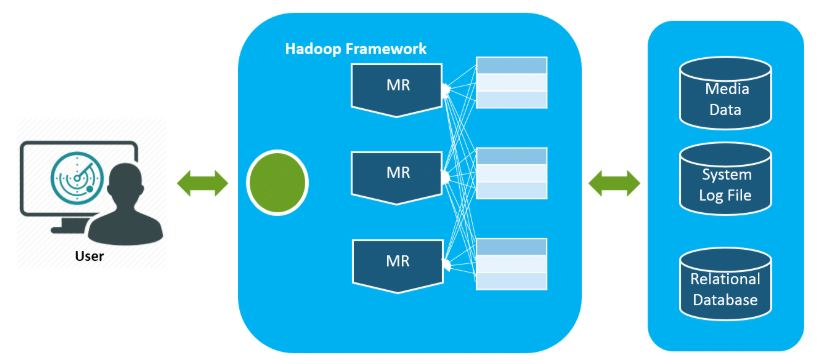
\includegraphics[scale=0.5]{hadoop_intro}
	\caption{Gambaran Umum Cara Kerja Hadoop}
	\label{fig:hadoop_intro}
\end{figure}

\noindent Hadoop memiliki karakteristik sebagai berikut:
\begin{itemize}
\item Hadoop menyediakan penyimpanan HDFS dan menggunakan pemodelan MapReduce.
\item Hadoop melakukan replikasi data sejenis pada beberapa komponen berbeda. 
\item Hadoop fleksibel terhadap pengaturan jumlah komponen yang bekerja.
\item Hadoop dioptimalkan untuk bekerja pada lingkungan big data.
\item Hadoop menulis data sekali dan membaca data berulang kali.

\end{itemize}

\subsection{Ekosistem Hadoop}
\begin{figure}[H]
	\centering
	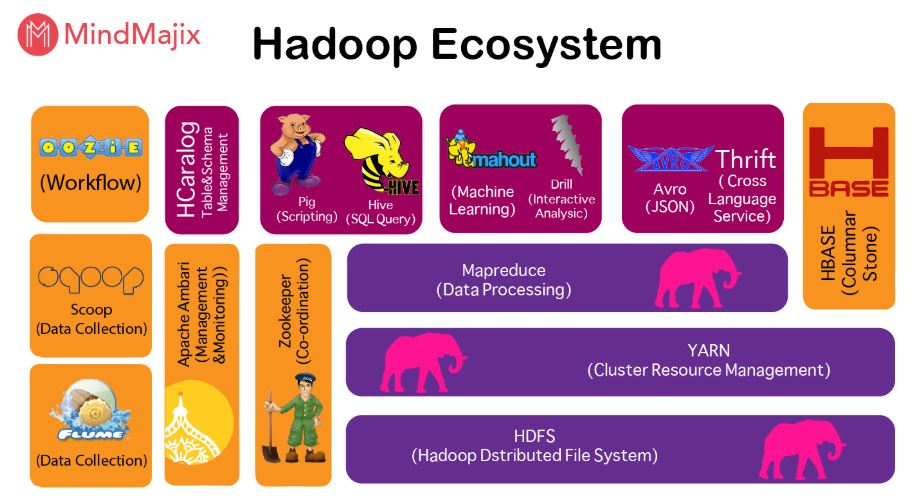
\includegraphics[scale=0.65]{hadoop_ecosystem}
	\caption{Ekosistem Hadoop}
	\label{fig:hadoop_ecosystem}
\end{figure}
Gambar \ref{fig:hadoop_ecosystem} menunjukan bahwa Hadoop dapat bekerja secara bersamaan dengan teknologi big data lainnya seperti Spark, HBase, Cassandra, STORM, dan lain-lain untuk memenuhi berbagai macam kebutuhan dalam pengolahan dan analisis pada big data.

\subsection{Arsitektur Hadoop}
\begin{figure}[H]
	\centering
	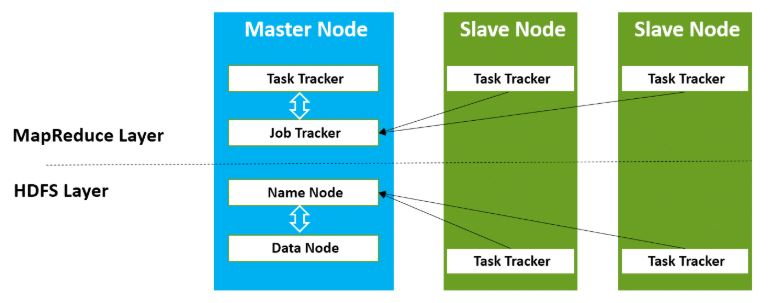
\includegraphics[scale=0.7]{arsitektur_hadoop}
	\caption{Arsitektur Hadoop}
	\label{fig:arsitektur_hadoop}
\end{figure}
Gambar \ref{fig:arsitektur_hadoop} menunjukan arsitektur Hadoop yang tersusun atas MapReduce dan Hadoop Distributed File System (HDFS). Masing-masing bagian memiliki dua jenis node yaitu master node dan slave node. Master node mengatur jumlah pekerjaan yang diberikan kepada dirinya sendiri dan slave node. Slave node mengerjakan pekerjaan yang diberikan oleh master node.


\subsection{HDFS}
HDFS adalah sistem file terdistribusi pada Hadoop dengan menyediakan penyimpanan data yang handal, mendukung partisi, dan toleran terhadap kesalahan pada hardware. HDFS bekerja erat dengan MapReduce dengan mendistribusikan penyimpanan dan perhitungan di seluruh cluster dengan menggabungkan sumber daya penyimpanan yang dapat dipartisi tergantung kebutuhan. 
\\\\
Lapisan penyimpanan HDFS terdiri dari dua elemen:

\begin{itemize}
\item NameNode\\
NameNode adalah sebuah komputer yang bertindak sebagai master node, sedangkan. NameNode bertanggungjawab menyimpan informasi tentang penempatan block-block data dalam Hadoop Cluster. Ia bertanggungjawab mengorganisir dan mengontrol block-block data yang disimpan tersebar dalam komputer-komputer yang menyusun Hadoop Cluster. 

\item DataNode\\
DataNode adalah elemen penyimpanan utama HDFS yang menyimpan blok data dan permintaan baca / tulis layanan pada file yang disimpan di HDFS. DataNode dikendalikan oleh NameNode. Blok yang disimpan dalam DataNodes direplikasi sesuai konfigurasi untuk memberikan keandalan dan ketersediaan tinggi. Blok yang direplikasi ini didistribusikan di seluruh cluster untuk memberikan perhitungan yang cepat.
\end{itemize}

\subsection{MapReduce}
MapReduce adalah kerangka kerja pemrograman untuk komputasi terdistribusi yang dibuat oleh Google menggunakan membagi dan menaklukkan metode untuk memecah masalah data besar yang kompleks menjadi unit-unit kecil pekerjaan dan memprosesnya sejajar. Model pemrograman Map Reduce terdiri dari dua fungsi, yaitu Mapper dan Reducer. 

\begin{figure}[H]
	\centering
	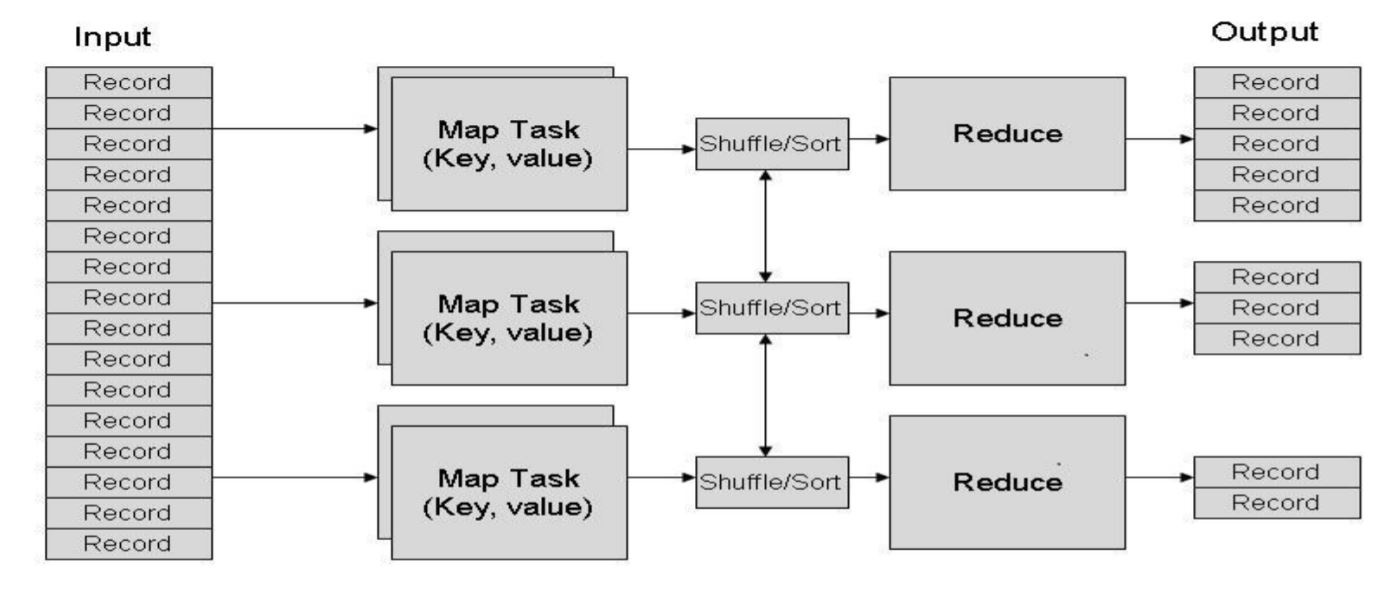
\includegraphics[scale=0.4]{MapReduceImage}
	\caption{Tahapan pada MapReduce}
	\label{fig:MapReduceImage}
\end{figure}

\noindent Pada Gambar \ref{fig:MapReduceImage}, tahapan MapReduce dapat dibagi menjadi dua fungsi utama:

\begin{itemize}
\item Mapper\\
Tugas fungsi Mapper adalah memetakan blok data kedalam pasangan <key,value>. Key,value pada Mapper tidak harus memiliki tipe data yang sama satu sama lain. Pasangan <key,value> yang mungkin terjadi pada fungsi Mapper adalah tidak memiliki pasangan atau memiliki banyak pasangan.

\item Reducer\\
Reducer memiliki 3 fase utama: shuffle, sort dan reducer. Berikut adalah penjelasan dari tahapan yang dilakukan oleh fungsi Reducer:

\begin{enumerate}
\item Shuffle \\
Shuffle adalah fase pada data antara untuk menggabungkan semua nilai menjadi koleksi yang terkait dengan kunci yang sama.
\item Sort \\
Pasangan <key,value> pada satu node secara otomatis diurutkan oleh Hadoop sebelum diberikan kepada Reducer. Penyortiran dilakukan berdasarkan keterurutan nilai key. 
\item Reducer \\
Data output mapper yang diacak dan diurutkan disediakan untuk Reducer. Tahap ini membuat pasangan <key, (list of value)> baru berdasarkan pengelompokan key.
\end{enumerate}

\end{itemize}

\noindent Berikut adalah komponen yang mengatur pekerjaan pada MapReduce:

\begin{itemize}
\item JobTracker\\
JobTracker berjalan pada master node untuk memonitor tugas-tugas MapReduce yang telah dijalankan oleh TaskTracker pada node salve. Tugas JobTracker adalah mengalokasikan pekerjaan yang sesuai untuk TaskTracker tertentu tergantung pada berapa banyak slot tugas yang tersedia. 
\item TaskTracker\\
TaskTracker berjalan pada masing-masing node slave. TaskTracker menerima pekerjaan dari JobTracker dan menjalankan operasi MapReduce. Setiap TaskTracker memiliki jumlah slot pekerjaan yang terbatas. TaskTracker mengatur pelaksanaan setiap operasi MapReduce pada setiap node slave. 
\end{itemize}

\section{Spark} 
Spark adalah teknologi komputasi cluster kilat-cepat, yang dirancang untuk komputasi cepat. Spark adalah paradigma pemrosesan data berukuran besar yang dikembangkan oleh para peneliti University of California di Berkeley. Spark adalah alternatif dari Hadoop MapReduce untuk mengatasi keterbatasan pemrosesan input output yang tidak efisien pada disk, dengan menggunakan memori. Fitur utama Spark adalah melakukan komputasi di dalam memori sehingga waktu komputasi menjadi lebih singkat dibandingkan waktu komputasi di dalam disk.
\\\\
Berikut adalah karakteristik dari Spark:
\begin{itemize}
\item Kecepatan\\
Spark adalah alat komputasi klaster tujuan umum. Ini menjalankan aplikasi hingga 100 kali lebih cepat dalam memori dan 10 kali lebih cepat pada disk daripada Hadoop. Spark mengurangi jumlah operasi baca/tulis pada disk dan menyimpan data dalam memori.


\item Mudah untuk diatur\\	
Spark dapat melakukan pemrosesan batch, analisis data secara interaktif, machine learning, dan streaming data. Semuanya pemrosesan tersebut dikerjakan pada satu komputer yang sama. Fungsi ini menjadikan Apache Spark sebagai mesin analisis data yang lengkap. 


\item Analisis secara real-time\\
Spark dapat dengan mudah memproses data waktu-nyata, misalnya streaming data secara real-time untuk ribuan peristiwa/detik. Contoh dari sumber streaming data adalah Twitter, Facebook, Instagram. Streaming data dapat diproses secara efisien oleh Spark.
\end{itemize}

\subsection{Ekosistem Spark}
\begin{figure}[H]
	\centering
	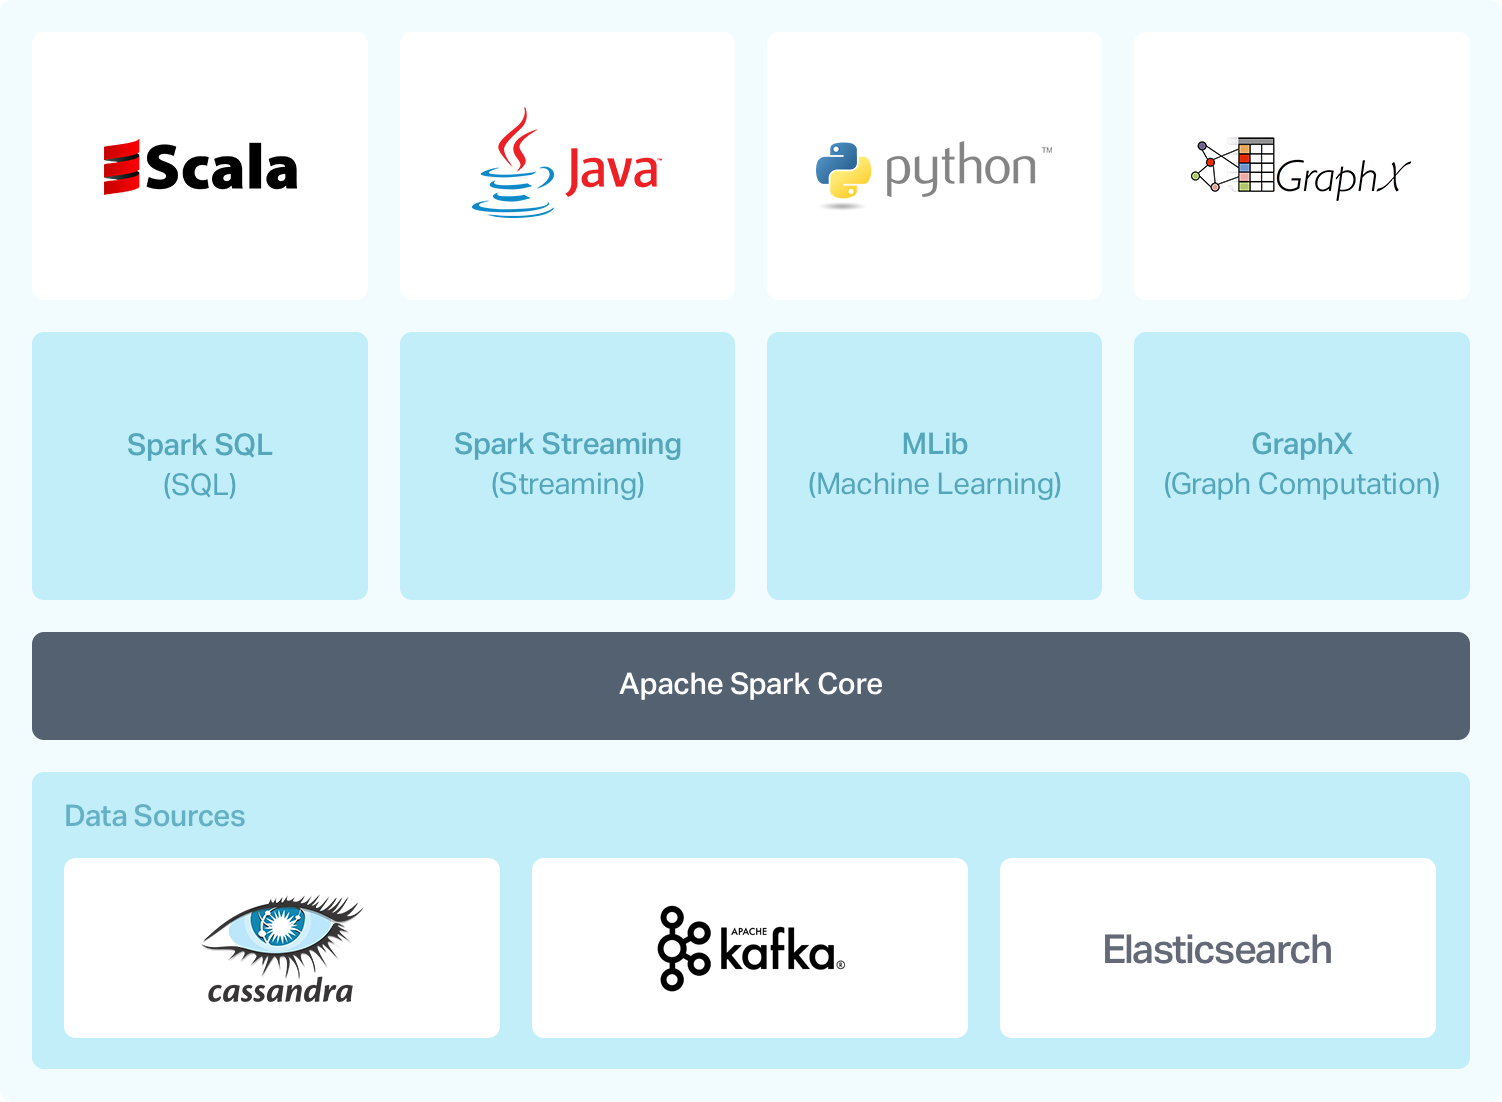
\includegraphics[scale=0.16]{spark_ecosystem}
	\caption{Ekosistem Spark}
	\label{fig:spark_ecosystem}
\end{figure}
Gambar \ref{fig:spark_ecosystem} menunjukan bahwa Spark bekerja sama dengan teknologi big data lain untuk memenuhi berbagai macam kebutuhan dalam pengolahan big data. Masing-masing warna pada Gambar \ref{fig:spark_ecosystem} mewakili jenis teknologi yang dipakai pada Spark. Spark SQL, Spark Streaming, Spark MLlib adalah library tambahan pada Spark. Cassandra, Kafka, dan ElasticSearch adalah framework untuk melakukan pengumpulan data secara streaming. Sedangkan scala, java, dan python adalah bahasa pemrograman yang dapat digunakan pada Spark.

\subsection{Arsitektur Spark}
\begin{figure}[H]
	\centering
	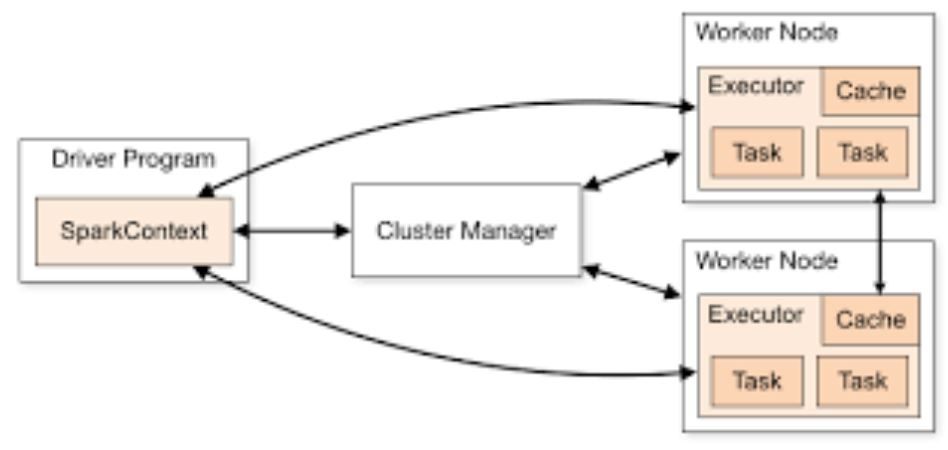
\includegraphics[scale=0.5]{arsitektur_spark2}
	\caption{Arsitektur Spark}
	\label{fig:arsitektur_spark2}
\end{figure}
Berikut adalah cara kerja pada arsitektur Spark:

\begin{enumerate}

\item
Program Driver memanggil program utama aplikasi dan membuat SparkContext dan Spark Driver. SparkContext terdiri dari semua fungsi dasar. Spark Driver berisi DAG Scheduler, Task Scheduler, Backend Scheduler, dan Block Manager.

\item
Spark Driver dan SparkContext secara kolektif mengawasi pelaksanaan pekerjaan di dalam cluster. Spark Driver bekerja sama dengan Cluster Manager untuk membagian pekerjaan ke setiap Worker Node. Setiap kali RDD dibuat dalam SparkContext, RDD akan didistribusikan di setiap Worker Node.

\item
Worker Node menjalankan tugas yang diberikan oleh Cluster Manager dan mengembalikannya ke Konteks Spark. Worker Node bertanggung jawab atas pelaksanaan tugas-tugas ini. Masa pakai pelaksana sama dengan masa hidup Aplikasi Spark. Jika ingin meningkatkan kinerja sistem, maka dapat meningkatkan jumlah pekerja sehingga pekerjaan dapat dibagi menjadi bagian kecil.

\end{enumerate}


\subsection{Jenis Instalasi pada Spark}
\begin{figure}[H]
	\centering
	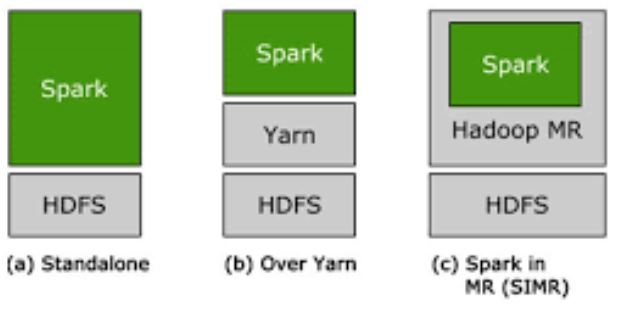
\includegraphics[scale=0.65]{arsitektur_spark}
	\caption{Arsitektur Spark}
	\label{fig:arsitektur_spark}
\end{figure}

Berikut adalah penjelasan jenis instalasi Spark pada Gambar \ref{fig:arsitektur_spark} sebagai berikut:

\begin{itemize}
\item Standalone\\  
Spark berdiri diatas HDFS Hadoop. Spark memungkinkan untuk mengakses data pada HDFS Hadoop untuk membaca input dan menulis output.

\item Hadoop Yarn\\
Spark dapat berjalan pada Hadoop Yarn tanpa memerlukan instalasi atau meminta hak akses root apapun. Hadoop Yarn membantu integrasi Spark pada ekosistem Hadoop.

\item Spark In MapReduce (SIMR)\\ 
SIMR digunakan untuk menjalankan pekerjaan Spark secara independen. Jenis instalasi ini sudah tidak lagi berlaku untuk Spark versi 2.0
\end{itemize}

\subsection{Resilient Distibuted Datasets (RDD)}
\par RDD adalah unit data logis utama di Spark. Mereka adalah kumpulan objek terdistribusi, yang disimpan dalam memori atau pada disk dari berbagai mesin cluster. RDD dapat dibagi menjadi beberapa partisi data sehingga partisi ini dapat disimpan dan diproses pada komputer yang berbeda. RDD adalah struktur data yang immutable (hanya baca). Anda tidak dapat mengubah RDD asli, tetapi Anda dapat membuat RDD baru dengan melakukan operasi butiran kasar, seperti transformasi, pada RDD yang ada. RDD dalam Spark dapat di simpan dalam cache dan digunakan lagi untuk transformasi di masa depan. RDD dievaluasi secara lazy, artinya Spark menunda evaluasi sampai benar-benar diperlukan. Ini menghemat banyak waktu dan meningkatkan efisiensi.

\begin{figure}[H]
	\centering
	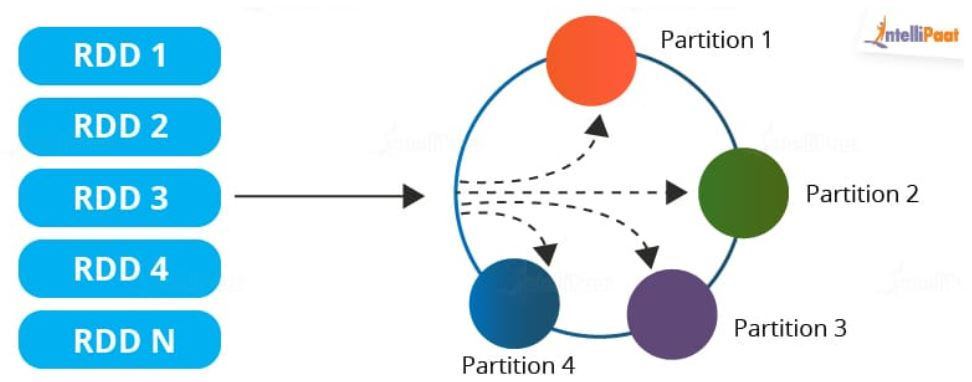
\includegraphics[scale=0.3]{rdd_intro}
	\caption{Cara Kerja RDD}
	\label{fig:rdd_intro}
\end{figure}

\subsubsection{Fitur pada RDD}
\noindent Berikut adalah fitur RDD pada Spark:
\begin{itemize}
\item Resilience: RDD melacak informasi garis keturunan data untuk memulihkan data yang hilang, secara otomatis jika gagal. Ini juga disebut toleransi kesalahan.

\item Distributed: Data yang ada dalam RDD berada di beberapa node. Ini didistribusikan di berbagai node cluster.

\item Lazy evaluation: Data tidak dimuat dalam RDD bahkan jika Anda mendefinisikannya. Transformasi sebenarnya dihitung ketika Anda memanggil suatu tindakan, seperti menghitung atau mengumpulkan, atau menyimpan output ke sistem file

\item Immutability: Data yang disimpan dalam RDD berada dalam mode read-only. RDD tidak dapat mengubah data didalamnya. Namun, RDD baru dapat dibuat dengan memanggil operasi transformasi pada RDD yang ada.

\item In-memory computation: RDD menyimpan data langsung apa pun yang dihasilkan dalam memori (RAM) selain pada disk sehingga memberikan akses yang lebih cepat.

\item Partitioning: Partisi dapat dilakukan pada RDD yang ada untuk membuat bagian logis yang bisa berubah. Anda dapat mencapai ini dengan menerapkan transformasi pada partisi yang tersedia.
\end{itemize}

\begin{figure}[H]
	\centering
	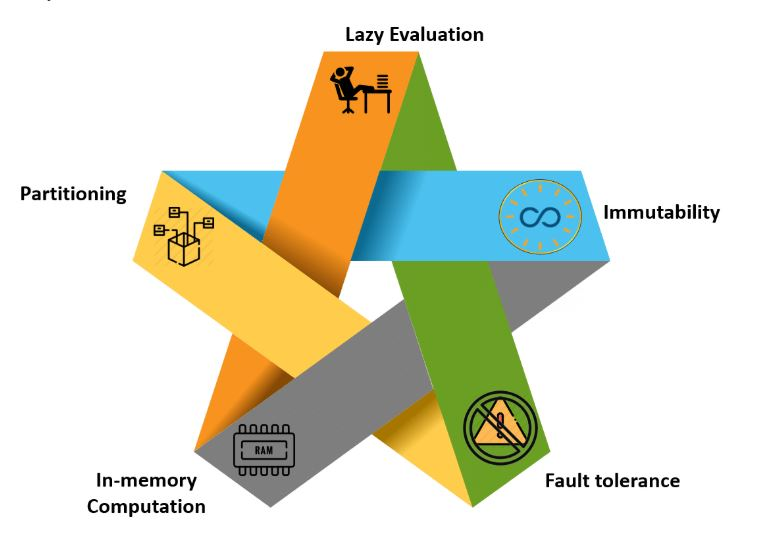
\includegraphics[scale=0.3]{rdd_feature}
	\caption{Fitur pada RDD}
	\label{fig:rdd_feature}
\end{figure}



\subsubsection{Operasi pada RDD}
\noindent Berikut adalah penjelasan singkat dan contoh dari jenis operasi pada RDD:

\begin{itemize}
\item Transformation\\
Tranformation adalah operasi pada RDD untuk mengembalikan output berupa RDD baru. Transformasi pada RDD dilakukan secara lazy, sehingga tranformasti hanya akan dikerjakan apabila dipanggil pada sebuah action. Transformasi pada RDD akan dijelaskan pada tabel dibawah ini.\\

\begin{tabular}{|l|p{10cm}|}
\hline 
\rule[-1ex]{0pt}{2.5ex} Fungsi & Deskripsi \\ 
\hline 
\rule[-1ex]{0pt}{2.5ex} map()	 & Mengembalikan RDD baru dengan menerapkan fungsi pada setiap elemen data \\ 
\hline 
\rule[-1ex]{0pt}{2.5ex} filter() & Mengembalikan RDD baru yang dibentuk dengan memilih elemen-elemen sumber di mana fungsi mengembalikan true \\ 
\hline 
\rule[-1ex]{0pt}{2.5ex} reduceByKey() & Menggabungkan nilai-nilai kunci menggunakan fungsi \\ 
\hline 
\rule[-1ex]{0pt}{2.5ex} groupByKey() & Mengonversi pasangan (kunci, nilai) menjadi pasangan (kunci, <iterable value>) \\ 
\hline 
\rule[-1ex]{0pt}{2.5ex} union() & Mengembalikan RDD baru yang berisi semua elemen dan argumen dari RDD sumber \\ 
\hline 
\rule[-1ex]{0pt}{2.5ex} intersection() & Mengembalikan RDD baru yang berisi persimpangan elemen dalam dataset \\ 
\hline 
\end{tabular} 

\item Action\\
Action adalah operasi yang mengembalikan nilai output ke dalam terminal atau melakukan penulisan data pada sistem penyimpanan eksternal. Action memaksa evaluasi pada RDD yang akan dipanggil, untuk menghasilkan output. Action pada RDD akan dijelaskan pada tabel dibawah ini.\\

\begin{tabular}{|l|p{10cm}|}
\hline 
\rule[-1ex]{0pt}{2.5ex} Fungsi & Deskripsi \\ 
\hline 
\rule[-1ex]{0pt}{2.5ex} count() & Mendapat jumlah elemen data dalam RDD \\ 
\hline 
\rule[-1ex]{0pt}{2.5ex} collect() & Mendapat semua elemen data dalam RDD sebagai array \\ 
\hline 
\rule[-1ex]{0pt}{2.5ex} reduce() & Agregat elemen data ke dalam RDD dengan mengambil dua argumen dan mengembalikan satu \\ 
\hline 
\rule[-1ex]{0pt}{2.5ex} take(n) & Mengambil n elemen pertama dari RDD \\ 
\hline 
\rule[-1ex]{0pt}{2.5ex} foreach(operation) & Menjalankan operasi untuk setiap elemen data dalam RDD \\ 
\hline 
\rule[-1ex]{0pt}{2.5ex} first() & Mengambil elemen data pertama dari RDD \\ 
\hline 
\end{tabular} 
\end{itemize}
 
\subsection{Komponen Spark}
Komponen Spark adalah library tambahan pada Spark untuk melakukan proses komputasi pada lingkungan big data berdasarkan jenis-jenis kebutuhan pengolahan data. Pada umumnya, Spark hanya membutuhkan library Spark Core saja untuk melakukan komputasi sederhana seperti pemrosesan pada MapReduce. Untuk kasus-kasus tambahan seperti implementasi kueri SQL dan teknik data mining digunakan library tambahan yaitu Spark Core dan Spark SQL. 
\\\\
Berikut adalah penjelasan singkat mengenai komponen pada Spark:

\begin{itemize}
\item Spark Core \\
Spark Core adalah library Spark yang berisi fungsionalitas dasar Spark, termasuk komponen untuk penjadwalan tugas, manajemen memori, pemulihan kesalahan, dan berinteraksi dengan sistem penyimpanan. Spark Core terdiri dari mesin eksekusi umum untuk platform Spark yang dibangun sesuai kebutuhan. Spark Core memberikan komputasi pada memori dan set data disimpan dalam sistem penyimpanan eksternal. Spark Core juga  menyediakan operasi action dan transformation pada RDD.

\item Spark SQL  \\
Spark SQL adalah komponen di atas Spark Core yang memperkenalkan serangkaian abstraksi data baru yang disebut SchemaRDD. SchemaRDD menyediakan dukungan untuk data terstruktur dan semi-terstruktur. Spark SQL memungkinkan pemrosesan kueri SQL pada lingkungan big data. Spark SQl menyediakan fungsi untuk menghitung nilai statistik dasar seperti mean, median, modus, nilai maksimum dan nilai minimum.

\item Spark Streaming \\
Spark Streaming adalah salah satu komponen Apache Spark, yang memungkinkan Spark dapat memproses data streaming secara real-time. Spark Streaming menyediakan API untuk memanipulasi aliran data yang cocok dengan RDD. Hal ini memungkinkan analisis data untuk beralih melalui sumber aplikasi yang memberikan data secara real time. Mirip dengan Spark Core, Spark Streaming berusaha untuk membuat sistem toleran dan scalable

\item
Spark MLlib \\
Spark MLlib adalah library Spark yang berisi fungsionalitas yang umum digunakan pada Machine Learning (ML). Untuk mengimplementasikan teknik data mining pada lingkungan big data dibutuhkan library Spark MLlib.  Spark MLlib menyediakan berbagai jenis algoritma Machine Learning termasuk klasifikasi, regresi, pengelompokan/clustering. Spark MLlib juga menyediakan fungsi untuk menghitung nilai statistik dasar seperti nilai maksimum, minimum, mean, dan variansi.

\end{itemize}

\section{Spark MLlib}
Spark MLlib diciptakan untuk skalabilitas, dan integrasi yang mudah dengan komponen pada Spark. Dengan adanya kemudahan tersebut diharapkan penelitan dapat difokuskan pada masalah pada pemodelan data daripada menyelesaikan masalah kompleksitas data. Spark MLlib adalah library pembelajaran mesin berdasarkan komputasi secara paralel. MLlib terdiri dari algoritma pembelajaran umum seperti klasifikasi,  pengelompokan/clustering. Spark MLLib dapat terintegrasi dengan komponen Spark lainnya seperti Spark SQL dan Spark Streaming. Spark MLlib dapat digunakan pada bahasa pemrograman Java, Scala, dan Python. Secara garis besar, MLlib melakukan data preprocessing, pelatihan model, dan membuat prediksi.
\\\\
Berikut adalah garis besar pekerjaan yang dilakukan oleh Spark MLlib:

\begin{enumerate}
\item Membuat RDD baru untuk merepresentasikan jenis fitur dalam dataset.
\item Melakukan ekstraksi fitur pada sebuah vektor dan konversi menjadi data numerik.
\item Menjalankan algoritma machine learning untuk menghasilkan pemodelan baru.
\item Melakukan evaluasi model dengan memanggil fungsi evaluasi milik Spark MLlib.
\end{enumerate}

\noindent Berikut adalah contoh pemodelan Spark MLlib yang umum digunakan untuk prediksi:

\begin{itemize}
\item Naive Bayes (klasifikasi)
\item K-Means (pengelompokan/clutering)
\item Statistika dasar (mean, variansi, nilai maksimum dan minimum)
\item Grafik (visualisasi data)
\end{itemize}

\subsection{Machine Learning pada Spark MLlib}

\begin{figure}[H]
	\centering
	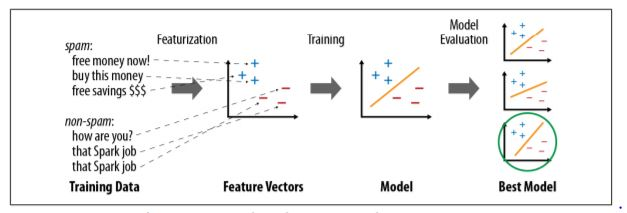
\includegraphics[scale=1.2]{machinelearningmllib}
	\caption{Tahapan Pembelajaran Machine Learning}
	\label{fig:machinelearningmllib}
\end{figure}
Algoritma pembelajaran mesin berupaya membuat prediksi atau keputusan berdasarkan data pelatihan. Ada beberapa jenis masalah pembelajaran termasuk klasifikasi, regresi, atau pengelompokan, yang memiliki tujuan yang berbeda. Semua algoritma pembelajaran membutuhkan pendefinisian sekumpulan fitur untuk setiap item, yang akan dimasukkan ke dalam fungsi pembelajaran. Sebagian besar algoritma didefinisikan hanya untuk fitur numerik (khususnya, vektor angka yang mewakili nilai untuk setiap fitur).
\\\\
\noindent Berikut adalah tahapan pembelajaran machine learning pada Spark MLlib sebagai berikut:

\begin{enumerate}

\item Featurization\\
Setelah data telah dibersihkan dan dipilih untuk pelatihan, perlu diubah menjadi representasi numerik dalam bentuk vektor sebagai input untuk model. Proses ini disebut vektorisasi. Proses pemilihan fitur yang tepat berpengaruh terhadap hasil pelatihan.
 
\item Training\\
Pelatihan model merupakan salah satu tahapan yang paling memakan waktu dan padat karya dalam setiap alur kerja pembelajaran mesin. Terlebih lagi, perangkat keras dan infrastruktur yang digunakan untuk melatih model sangat bergantung pada jumlah parameter dalam model, ukuran dataset, metode pengoptimalan yang digunakan, dan pertimbangan lainnya.

\item Model Evaluation\\
Setiap model harus menjalani evaluasi kualitatif dan kuantitatif. Banyak data pelatihan yang memiliki hasil evaluasi yang sesuai terhadap kinerja model. Model tersebut harus diterapkan pada data baru. Seringkali, pemeriksaan kualitatif tentang kinerja model, diperoleh dengan referensi silang prediksi model dengan apa yang diharapkan secara intuitif, dapat berfungsi sebagai panduan apakah model bekerja sesuai harapan.
\end{enumerate}

\subsection{Tipe Data pada Spark MLlib}
Spark MLlib terdiri dari beberapa jenis tipe data berdasarkan library bahasa pemrograman yang digunakan. Pada Java/Scala, library MLlib menggunakan istilah package. Pada Python, library MLlib menggunakan istilah pyspark.mllib. Tipe data Spark MLlib dibuat dengan cara menyimpan objek data RDD berdasarkan operasi tranformasi RDD pada dataset. \\\\

\newpage
\noindent Berikut adalah beberapa jenis tipe data pada Spark MLlib:

\begin{itemize}
\item Vektor\\
Vektor terdiri dari dua jenis yaitu vektor dense dan vektor sparse. Perlu digaris bawahi bahwa elemen vektor dense dan vektor sparse disimpan dalam struktur data array bertipe double. Kelas vektor berada pada package mllib.linalg.Vectors. Berikut adalah penjelasan singkat dari vektor dense dan vektor sparse:

\begin{itemize}

\item Vektor dense\\
Vektor dense adalah vektor yang menyimpan setiap nilai fitur dataset. Jumlah elemen pada vektor dense akan memiliki jumlah yang sama dengan jumlah fitur pada dataset. \\

\item Vektor sparse\\
Vektor sparse biasanya lebih disukai karena memiliki kelebihan dalam hal penggunaan memori dan kecepatan. Vektor sparse adalah vektor yang menyimpan setiap nilai fitur yang bukan nol pada dataset, sehingga jumlah elemen yang disimpan pada vektor sparse lebih sedikit dibandingkan dengan jumlah elemen yang disimpan pada vektor dense. 

\end{itemize}

\item LabeledPoint\\
LabeledPoint digunakan pada algoritma supervised learning yaitu klasifikasi dan regresi. LabeledPoint terdiri dari vektor fitur dan label yang direpresentasikan dengan tipe data Double. LabeledPoint terletak pada package "mllib.regress".

\item Various Model classes\\
Various Model classes adalah tipe data yang dihasilkan dari penerapan algoritma machine learning. Tipe data ini memiliki fungsi predict() untuk menerapkan pemodelan yang ada ke dalam data baru.

\end{itemize}

\subsection{Jenis Pemodelan pada Spark MLlib}

\subsubsection{Naive Bayes}

Naive Bayes adalah algoritma klasifikasi multiclass sederhana dengan asumsi independensi antara setiap pasangan fitur. Naive Bayes dapat dilatih dengan sangat efisien. Naive Bayes menghitung distribusi probabilitas bersyarat dari setiap fitur yang diberikan label, kemudian menerapkan teorema Bayes untuk menghitung distribusi probabilitas bersyarat label yang diberikan pengamatan dan menggunakannya untuk prediksi. Naive Bayes membutuhkan RDD dari LabeledPoint. Pemodelan Naive Bayes dapat digunakan untuk evaluasi dan prediksi. 
 

\subsubsection{K-Means}
K-Means adalah salah satu algoritma pengelompokan yang paling umum digunakan untuk mengelompokkan titik-titik data menjadi sejumlah kelompok yang telah ditentukan. K-Means memiliki parameter masukan sebagai berikut:

\begin{itemize}
\item \textit{k} adalah jumlah cluster yang diinginkan. 
\item \textit{maxIterations} adalah jumlah iterasi maksimum yang harus dijalankan.
\item \textit{initializationMode} menentukan inisialisasi centroid secara acak.
\item \textit{initializationSteps} menentukan jumlah langkah dalam algoritma k-means.
\item \textit{initialModel} adalah menentukan nilai centroid saat inisialisasi.
\end{itemize}

\section{Scala}
Scala adalah bahasa pemrograman berbasi open source, dibuat oleh Profesor Martin Odersky. Scala adalah bahasa pemrograman multi-paradigma dan mendukung paradigma fungsional serta berorientasi objek. Spark ditulis dalam Scala dan karena skalabilitasnya di JVM. Pemrograman scala adalah bahasa pemrograman yang paling banyak digunakan, oleh pengembang big data untuk mengerjakan proyek Spark. Untuk pengembangan Spark, penulisan sintaks Scala dianggap produktif untuk mengimplementasikan kode program. Pemrograman pada Scala mempertahankan prinsip keseimbangan antara produktivitas pengembangan program dan kinerja program. Pemrograman pada Scala tidak serumit pemrograman pada Java. Satu baris kode program pada Scala dapat menggantikan 20 hingga 25 baris kode java. Karena alasan terbut, Scala menjadi bahasa pemrograman yang sangat diminati untuk melakukan pemrosesan big data pada Spark.

\section{Scala Swing} 
Scala Swing adalah program berbasis Graphical User Interface (GUI) sehingga memiliki perbedaan dengan program Spark yang dieksekusi dengan terminal. Scala Swing bertujuan untuk memberi tampilan program sehingga hasil program diharapkan menjadi lebih interaktif. Scala menyediakan akses langsung terhadap kelas GUI pada Java menggunakan library Scala Swing.  Dengan menggunakan Scala, penggunaan Scala Swing dapat memenuhi kebutuhan perancangan User Interface melalui berbagai macam komponen GUI pada umumnya. Gambar \ref{fig:swing_example} adalah contoh implementasi GUI sederhana pada Scala Swing.

\begin{figure}[H]
	\centering
	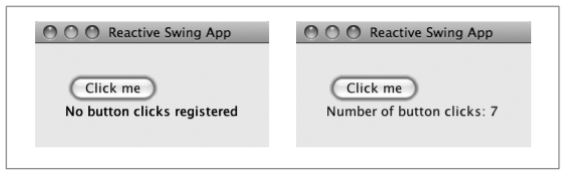
\includegraphics[scale=0.75]{swing_example}
	\caption{GUI Sederhana pada Scala Swing}
	\label{fig:swing_example}
\end{figure}


\subsection{Panel dan Layout}
Panel adalah tempat untuk menampilkan semua komponen GUI dengan beberapa aturan tata letak yang harus dipenuhi. Salah satu bagian tersulit pada perancangan aplikasi berbasis GUI adalah mengatur penempatan layout dengan benar. Gambar \ref{fig:swing_panel} diberikan sebagai contoh penerapan konsep dasar untuk menyusun aplikasi GUI. Layout dibangun atas beberapa komponen GUI seperti Frame, Panel, Label atau Button. Komponen ini memiliki nilai properti (warna, ukuran, posisi) yang dapat diatur secara manual.

\subsection{Handling Event}
Handling event adalah perkerjaan yang dilakukan masing-masing komponen. Komponen akan menerima aksi langsung dari pengguna aplikasi. Mekanisme ini dikenal sebagai handling event, yang dieksekusi ketika suatu peristiwa terjadi. Handling event memiliki listener. Listener adalah sebuah komponen memberi tahu sebuah aksi kepada komponen tertentu. Listener harus dibuat untuk masing-masing objek handling event. Gambar \ref{fig:swing_handle_event} adalah contoh implementasi handling event pada Scala Swing.

\section{Jenis Data Input}
Spark menerima berbagai jenis data input dan menfasilitasi penulisan berbagai jenis data output. Berberapa jenis data yang akan diolah memiliki format penulisan masing-masing, sehingga memiliki cara yang berbeda untuk mengambil dan menulis sekumpulan data dalam format tertentu. 

\subsection{CSV}
Comma Separated Value (CSV) berisi sejumlah jumlah atribut data untuk setiap baris dan dipisahkan oleh koma. CSV tidak memiliki format yang konsisten. CSV tidak dapat mengakses nilai atribut data secara langsung. Untuk mendapatkan nilai atribut secara spesifik, perlu dilakukan pemisahan koma untuk setiap baris data. Spark mampu melakukan proses manipulasi dan transformasi CSV tanpa menggunakan library tambahan.

\subsection{XML}
XML menyediakan format penulisan data menggunakan tag pembuka dan penutup. Tag pembuka dan penutup pada XML ditulis dengan tujuan memberi tahu data-data apa saja yang merupakan cakupan dari elemen tag tersebut. Dalam beberapa tahun terakhir, pengolahan data dengan format XML semakin meningkat seiring berkembangnya pemakaian XML sebagai format penyimpanan data. Spark mampu melakukan proses manipulasi dan transformasi data XML dengan menggunakan library tambahan.
